\documentclass[10pt,letterpaper,twocolumn]{IEEEtran}
\usepackage[utf8]{inputenc}
%\usepackage[brazil]{babel}
\usepackage[T1]{fontenc}
\usepackage{amsmath}
\usepackage{amsfonts}
\usepackage{amssymb}
\usepackage{graphicx}
\usepackage{cite}
\usepackage{indentfirst}
\usepackage[width=8.50in, height=11.00in, left=0.625in, right=0.625in, top=0.75in, bottom=1.00in]{geometry}
\author{Hiram Amaral}
\title{Sistema Inteligente Ágil de Processo Evolutivo - SIAPE: Um protótipo brasileiro de sistemas EPS}
\usepackage{keywords}
\usepackage{nomencl}
\usepackage{multirow}
\usepackage{array}
\usepackage{hhline}
\usepackage{rotating}
\newcolumntype{C}[1]{>{\centering\let\newline\\\arraybackslash\hspace{0pt}}m{#1}}
%=========================== DOCUMENTO =========================
\begin{document}
	
	
	%======================== autores e afiliações ========================
	\author{
		\IEEEauthorblockN{Hiram Amaral,
			\IEEEauthorrefmark{0} André  Luiz  Duarte Cavalcante
			\IEEEauthorrefmark{0} e Lucas Cordeiro
			\IEEEauthorrefmark{0}}
		\IEEEauthorblockA{
			\IEEEauthorrefmark{0}\\
			\textit {Universidade Federal do Amazonas  - Mestrado em Engenharia Elétrica}\\
			\textit {Av. General Rodrigo Octávio Jordão Ramos, 3000, Setor Norte, Coroado I -- Manaus, AM, Brasil}\\
			Email:  \{hiramaral, mendoncarms, andrecavalcane\}@ufam.edu.br } e  lucascordeiro@gmail.com	}
	%====================== Abstract =================================
	\maketitle
	\begin{abstract}
Paradigmas emergentes de fabricação têm sido usados na tentativa de solucionar o problema da customização, isto é, a manufatura de produtos em lotes baixos e com elevados níveis de variedades de produtos. Notadamente os \textit{Evolvable Production Systems (EPS)} tem conseguido tratar o problema através do conceito de agentes mecatrônicos e de uma inversão do local de onde a inteligência do processo produtivo está dentro do sistema de manufatura. Entretanto, ainda há várias lacunas e barreiras ao amplo uso de EPS, dentre elas a necessidade de protótipos de sistemas que contemplem os conceitos de sistemas evolutivos. Este trabalho apresenta o desenvolvimento de um sistema evolutivo denominado de Sistema Inteligente Ágil de Processo Evolutivo - SIAPE que visa adaptação à demanda e a evolução do sistema produtivo de acordo com a evolução do produto. Para testar a viabilidade do SIAPE foi criado primeiramente um protótipo de automação simplificado chamado de Produto UFAM que é comparado com o protótipo SIAPE propriamente dito em torno de suas aderências às exigências da Plataforma da Indústria 4.0 (i4.0).\par
		%====================== Keyworpds  =================================
		\begin{keywords}
			\it Automation manufacturing, Evolvable Production System, Industrie 4.0, CPS e MeDSE 
		\end{keywords}
	\end{abstract}
	
% SEÇÃO I
	\section{INTRODUÇÃO}
	%==================================
%==================================

Até o final da década de 80 os sistemas flexíveis conseguiam resolver o principal problema das empresas industriais até então: a produção em lotes médios e pequenos. Contudo, a partir de 1989, intensificou-se a troca de bens entre diferentes continentes e as exigências dos clientes levou ao aumento do nível de customização. Além disso, tecnologias como a Internet aproximaram mercados e consumidores de locais distantes. A troca rápida de informações e os ativos intangíveis transformaram a economia mundial numa rede global de conhecimento~\cite{E.Abele}.

Para fazer frente a esses novos desafios, naturalmente houve o desenvolvimento de novas formas de se olhar a manufatura. Essas novas forma são conhecidas como os paradigmas da manufatura cujos surgimentos estão ilustrados  na Figura~\ref{F5}. Nela estão enfatizados o paradigma \textit{Flexible Manufacturing System (FMS)} \cite{FMS} e o surgimento dos paradigmas emergentes \textit{(Holonic Manufacturing System (HMS) \cite{Christensen,VanBrussel}, Bionic Manufacturing System (BMS) \cite{BMS} e \textit{Reconfiguration Manufacturing System (RMS)} \cite{RMS})}. Esses paradigmas inovaram ao desconsiderar os equipamento da manufatura como detentores da inteligência para a montagem, isto é, o conhecimento do processo produtivo. Nesses paradigmas e, em especial no paradigma \textit{Evolvable Production System (EPS)} \cite{M.Onori_a}, o foco da inteligência foi direcionado para o produto, que detém o conhecimento da montagem de si mesmo e não mais as ferramentas de montagem. 

Também os sistemas evolutivos passam a ter, atualmente, maior relevância no tratamento do problema da customização e estão sendo testados objetivando as indústrias inteligentes e as exigências da Indústria 4.0 \cite{BITKOM2015,VDE2014}. 

 \begin{figure}[h!]
 	\centering
 	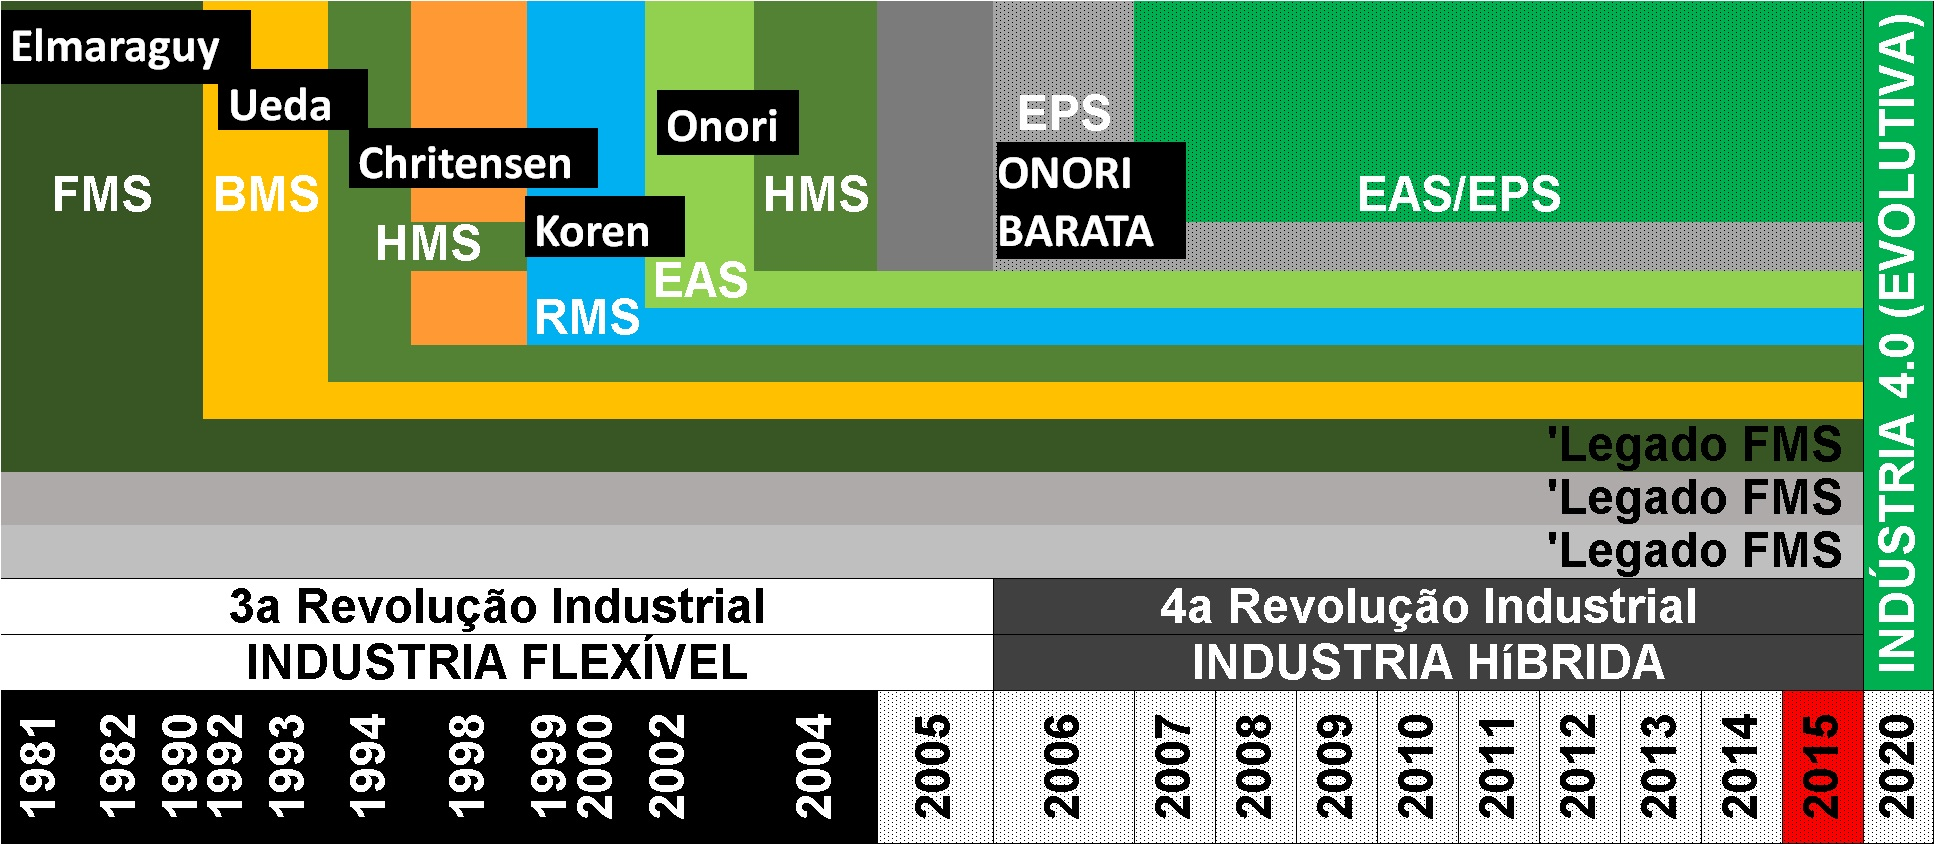
\includegraphics[width=8.9cm, height=4cm]{MeDSE_imagens/F7_MeDSE_PARAD1.jpg} 
 	\caption{Paradigmas de Produção}
 	\label{F5}
 \end{figure}

 Para mostrar a realização desta proposta de desenvolvimento e sua aplicação, este artigo está assim dividido: A seção II descreve as características dos sistemas \textit{EPS}; a seção III desenvolve a arquitetura e do Sistema Inteligente Ágil de Processo Evolutivo - SIAPE; Na seção IV o sistema é implementado e realiza uma experimentação; Na seção V os resultados são analisados e o sistema é validado; Na seção VI a conclusão e os trabalhos futuros são apresentados.
 
% SEÇÃO II
\section{SISTEMAS EVOLUTIVOS DE PRODUÇÃO -- EVOLVABLE PRODUCTION SYSTEM - EPS}



Os sistemas evolutivos são baseados em agentes inteligentes e autônomos que são capazes de cooperarem entre si. Esta
cooperação leva tais sistemas a possuírem a capacidade de adaptação e de evolução \cite{ROSA2013c}.
Por adaptação entende-se que o sistema é capaz de propor uma configuração alternativa de si mesmo para minimizar os
efeitos adversos de perturbações. Adaptação é de curto prazo e, normalmente, implica auto-reconfiguração na forma de ajustes
de parâmetros. Já o termo evolução refere-se ao sistema que é capaz de permitir a introdução ou remoção de módulos
existentes sem implicar na perda de performance e/ou quebra do seu funcionamento. A evolução se caracteriza num processo
de longo prazo, podendo o sistema evoluir até o limite da tecnologia ou ao da planta fabril. \par

Como um sistema evolutivo é baseado em agentes autônomos que reconhecem o ambiente físico e são capazes de
executar alguma ação sobre este ambiente, \textit{EPS} apresenta auto--organização, isto é, o sistema é capaz de reconhecer os agentes
que estiverem ativos em determinado momento e formar a sociedade de agentes necessária. Portanto, o paradigma \textit{EPS}
muda o foco da inteligência, no chão de fábrica, dos equipamentos que formam o sistema produtivo para o produto. Por
causa da sua arquitetura baseada em agentes inteligentes, que possuem a capacidade de auto-organização, possuem também
a propriedade do “plugar e produzir”.


 \subsection{CARACTERÍSTICAS DOS SISTEMAS EPS}

Os EPS possuem algumas características interessantes, pois possuem em um grau elevado, adaptabilidade, evolutibilidade, modularidade e sua granularidade pode ser ajustada conforme a complexidade do sistema. Para este trabalho, estes termos tem os seguintes significados:

\textbf{Adaptabilidade} -- o sistema tem de ser capaz de propor uma configuração alternativa para minimizar os efeitos adversos de perturbações. Adaptação é de curto prazo e, normalmente, implica \textit{auto-reconfiguração} na forma de ajustes de parâmetros~\cite{ROSA2013c}.

\textbf{Evolutibilidade} -- 
Em relação à \textit{evolução}, o sistema tem de ser capaz de permitir a introdução ou remoção de módulos existentes sem implicar na performance e no funcionamento do sistema. A evolução se caracteriza num processo de longo prazo, podendo o sistema evoluir até o limite da tecnologia ou ao limite da planta fabril~\cite{ROSA2013c}.

\textbf{Modularidade} -- denotada pela noção de independência entre os módulos dos sistema.

\textbf{Plugabilidade} -- se o sistema pode inserir ou remover módulos como parte de seu funcionamento normal em tempo de produção.

\textbf{Granularidade} -- que evidencia o quanto de informação um agente deve possuir sobre os demais agentes, e a quantidade destes, a fim de se conseguir um objetivo definido.

Para este texto, \textbf{reconfigurabilidade} é a habilidade do sistema de redesenhar seu layout sem comprometer o funcionamento do sistema. Portanto, a plugabilidade é uma espécie de reconfigurabilidade. 

Quando um sistema possuir algum grau desses parâmetros, ele é dito possuir a \textbf{auto-organização} e o sistema é dito ser \textbf{dinâmico}.


 \subsection{ARQUITETURA EPS DE REFERÊNCIA}
 
 
 EPS é baseado em agentes inteligentes. Nas primeiras arquiteturas havia a definição de muitos tipos diferentes de agentes, capazes de tratar certos aspectos do sistema produtivo, tais como transporte, acesso hardware ou agentes de coalizão. Atualmente, EPS pode ser descrito como uma abordagem multiagente capaz de auto-organização e execução de processos complexos através da interação entre os agentes que formam o sistema. Há basicamente dois tipos de agentes em EPS: os agentes mecatrônicos e os agentes não mecatrônicos. Dentre os agentes mecatrônicos, pode-se citar a existência de dois subtipos: agentes cognitivos e agentes motores. 
 
 A arquitetura de referência pode ser vista na Figura \ref{fig:arq_referencia_eps}, que mostra dois tipos de agentes mecatrônicos: agente de recurso e agente de coalizão. Agentes de produtos são um tipo de  agente de coalizão. Agentes de transporte são um tipo de agente mecatrônico normal, mas especializado no sistema de  transporte. Tais sistemas estão sendo desenvolvidos e testados objetivando as fábricas inteligentes e a padronização proposta pela  Plataforma \cite{BITKOM2015} da Indústria 4.0 \cite{DRATH2014}.
 
\begin{figure}[t]
	\centering
	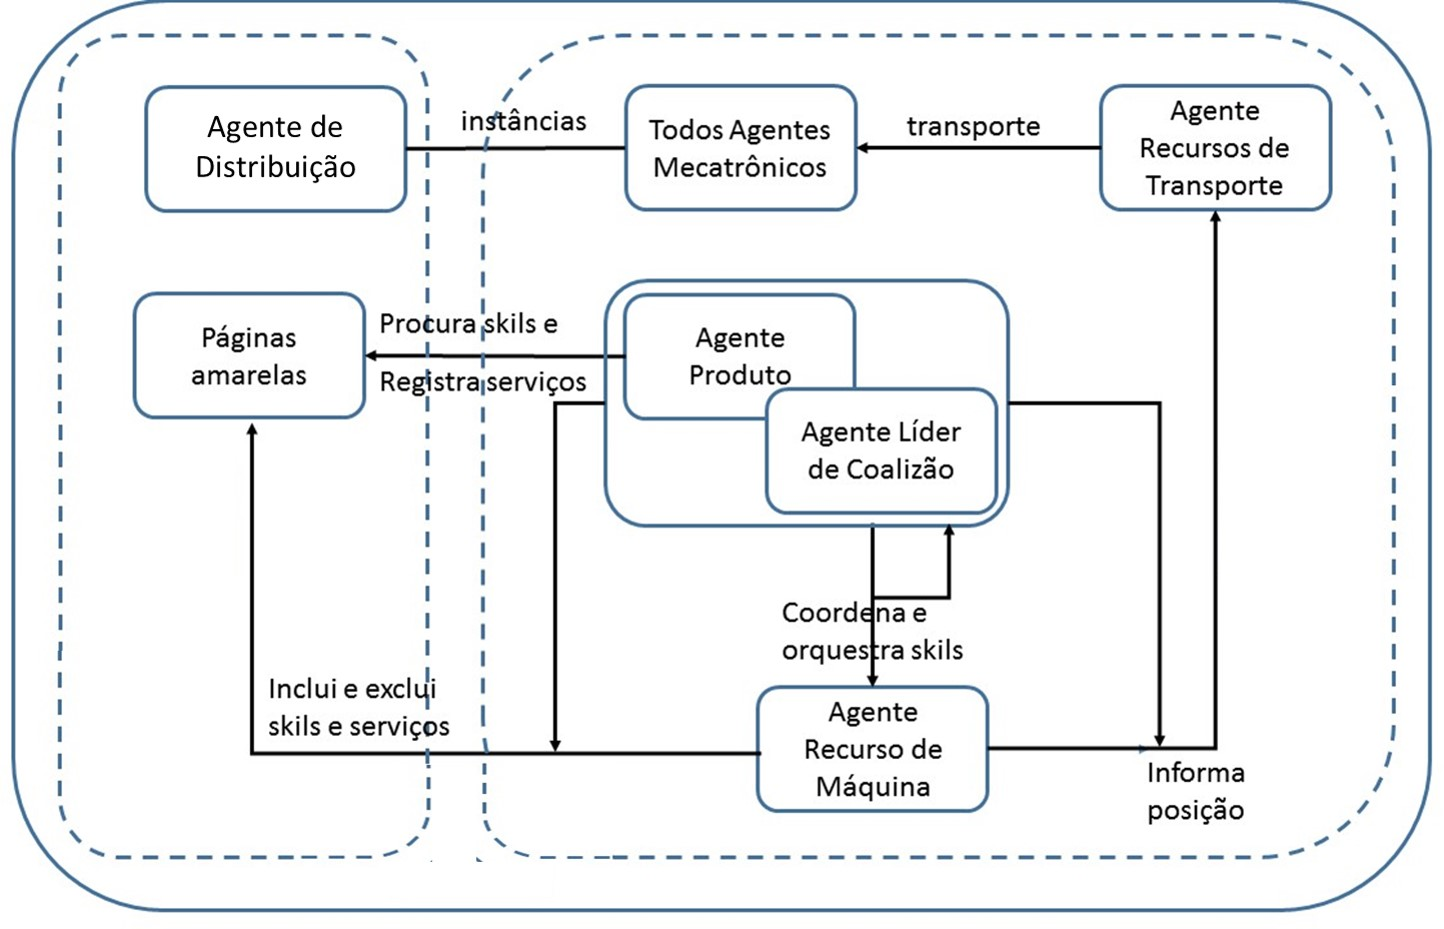
\includegraphics[width=8.9cm, height=6cm]{MeDSE_imagens/F8_1_SIAPE_Arquitetura_EPS.jpg}
	\caption{IADE: Arquitetura de referência \textit{EPS}}
	\label{fig:arq_referencia_eps}
	{\footnotesize{Fonte: \cite{A.L.D.Cavalcante}}}
\end{figure}

\subsection{ARQUITETURA EPS DE CAVALCANTE}

A arquitetura \textit{EPS} proposta por Cavalcante denominada de Arquitetura Baseada em Agentes e Auto-Organizável Para a Manufatura  está ilustrada na Figura \ref{F132} e é descrita a seguir.
\begin{figure}[h!]
	\centering
	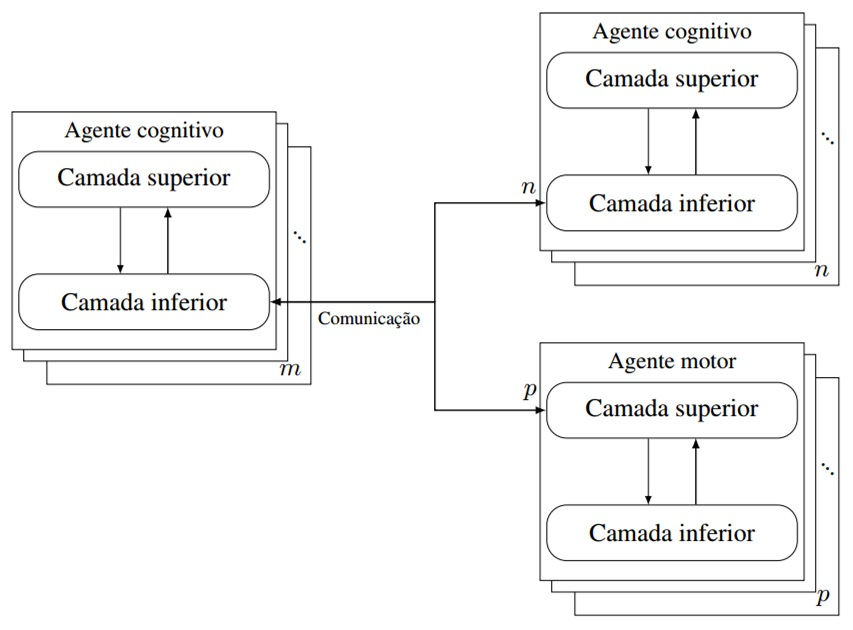
\includegraphics[width=8.9cm, height=5cm]{MeDSE_imagens/F132_ARQUITETURA_BAAOPM.jpg} 
	\caption{Visão geral da Arquitetura proposta por Cavalcante}
	\footnotesize{Fonte: \cite{A.L.D.Cavalcante}}
	\label{F132}
\end{figure}
A arquitetura é formada por dois tipos de agentes:
\textbf{O agente cognitivo} é o responsável pela lógica da aplicação empregada na situação e escolhe uma decisão a ser realizada, por outro agente cognitivo ou por um agente motor. A camada superior funciona como aplicação do agente e  a camada inferior funciona como interface de comunicação com os outros agentes do sistema, e promove a seleção e as requisições feitas para os outros agentes do sistema.

\textbf{O agente motor} por sua vez, tem sua camada superior funcionando como comunicação e a camada inferior como a aplicação do agente. A camada superior recebe a comunicação das operações a serem realizadas que são enviadas pelo agente cognitivo. A camada inferior além de ter a função da aplicação do agente, funciona como camada de sensoriamento percebendo o ambiente e informando as condições sentidas ao  cognitivo, para que este tome as decisões necessárias e as realize as tarefas atribuídas ao sistema.

\subsection{ARQUITETURA SIAPE}
\begin{figure}[b]
	\centering
	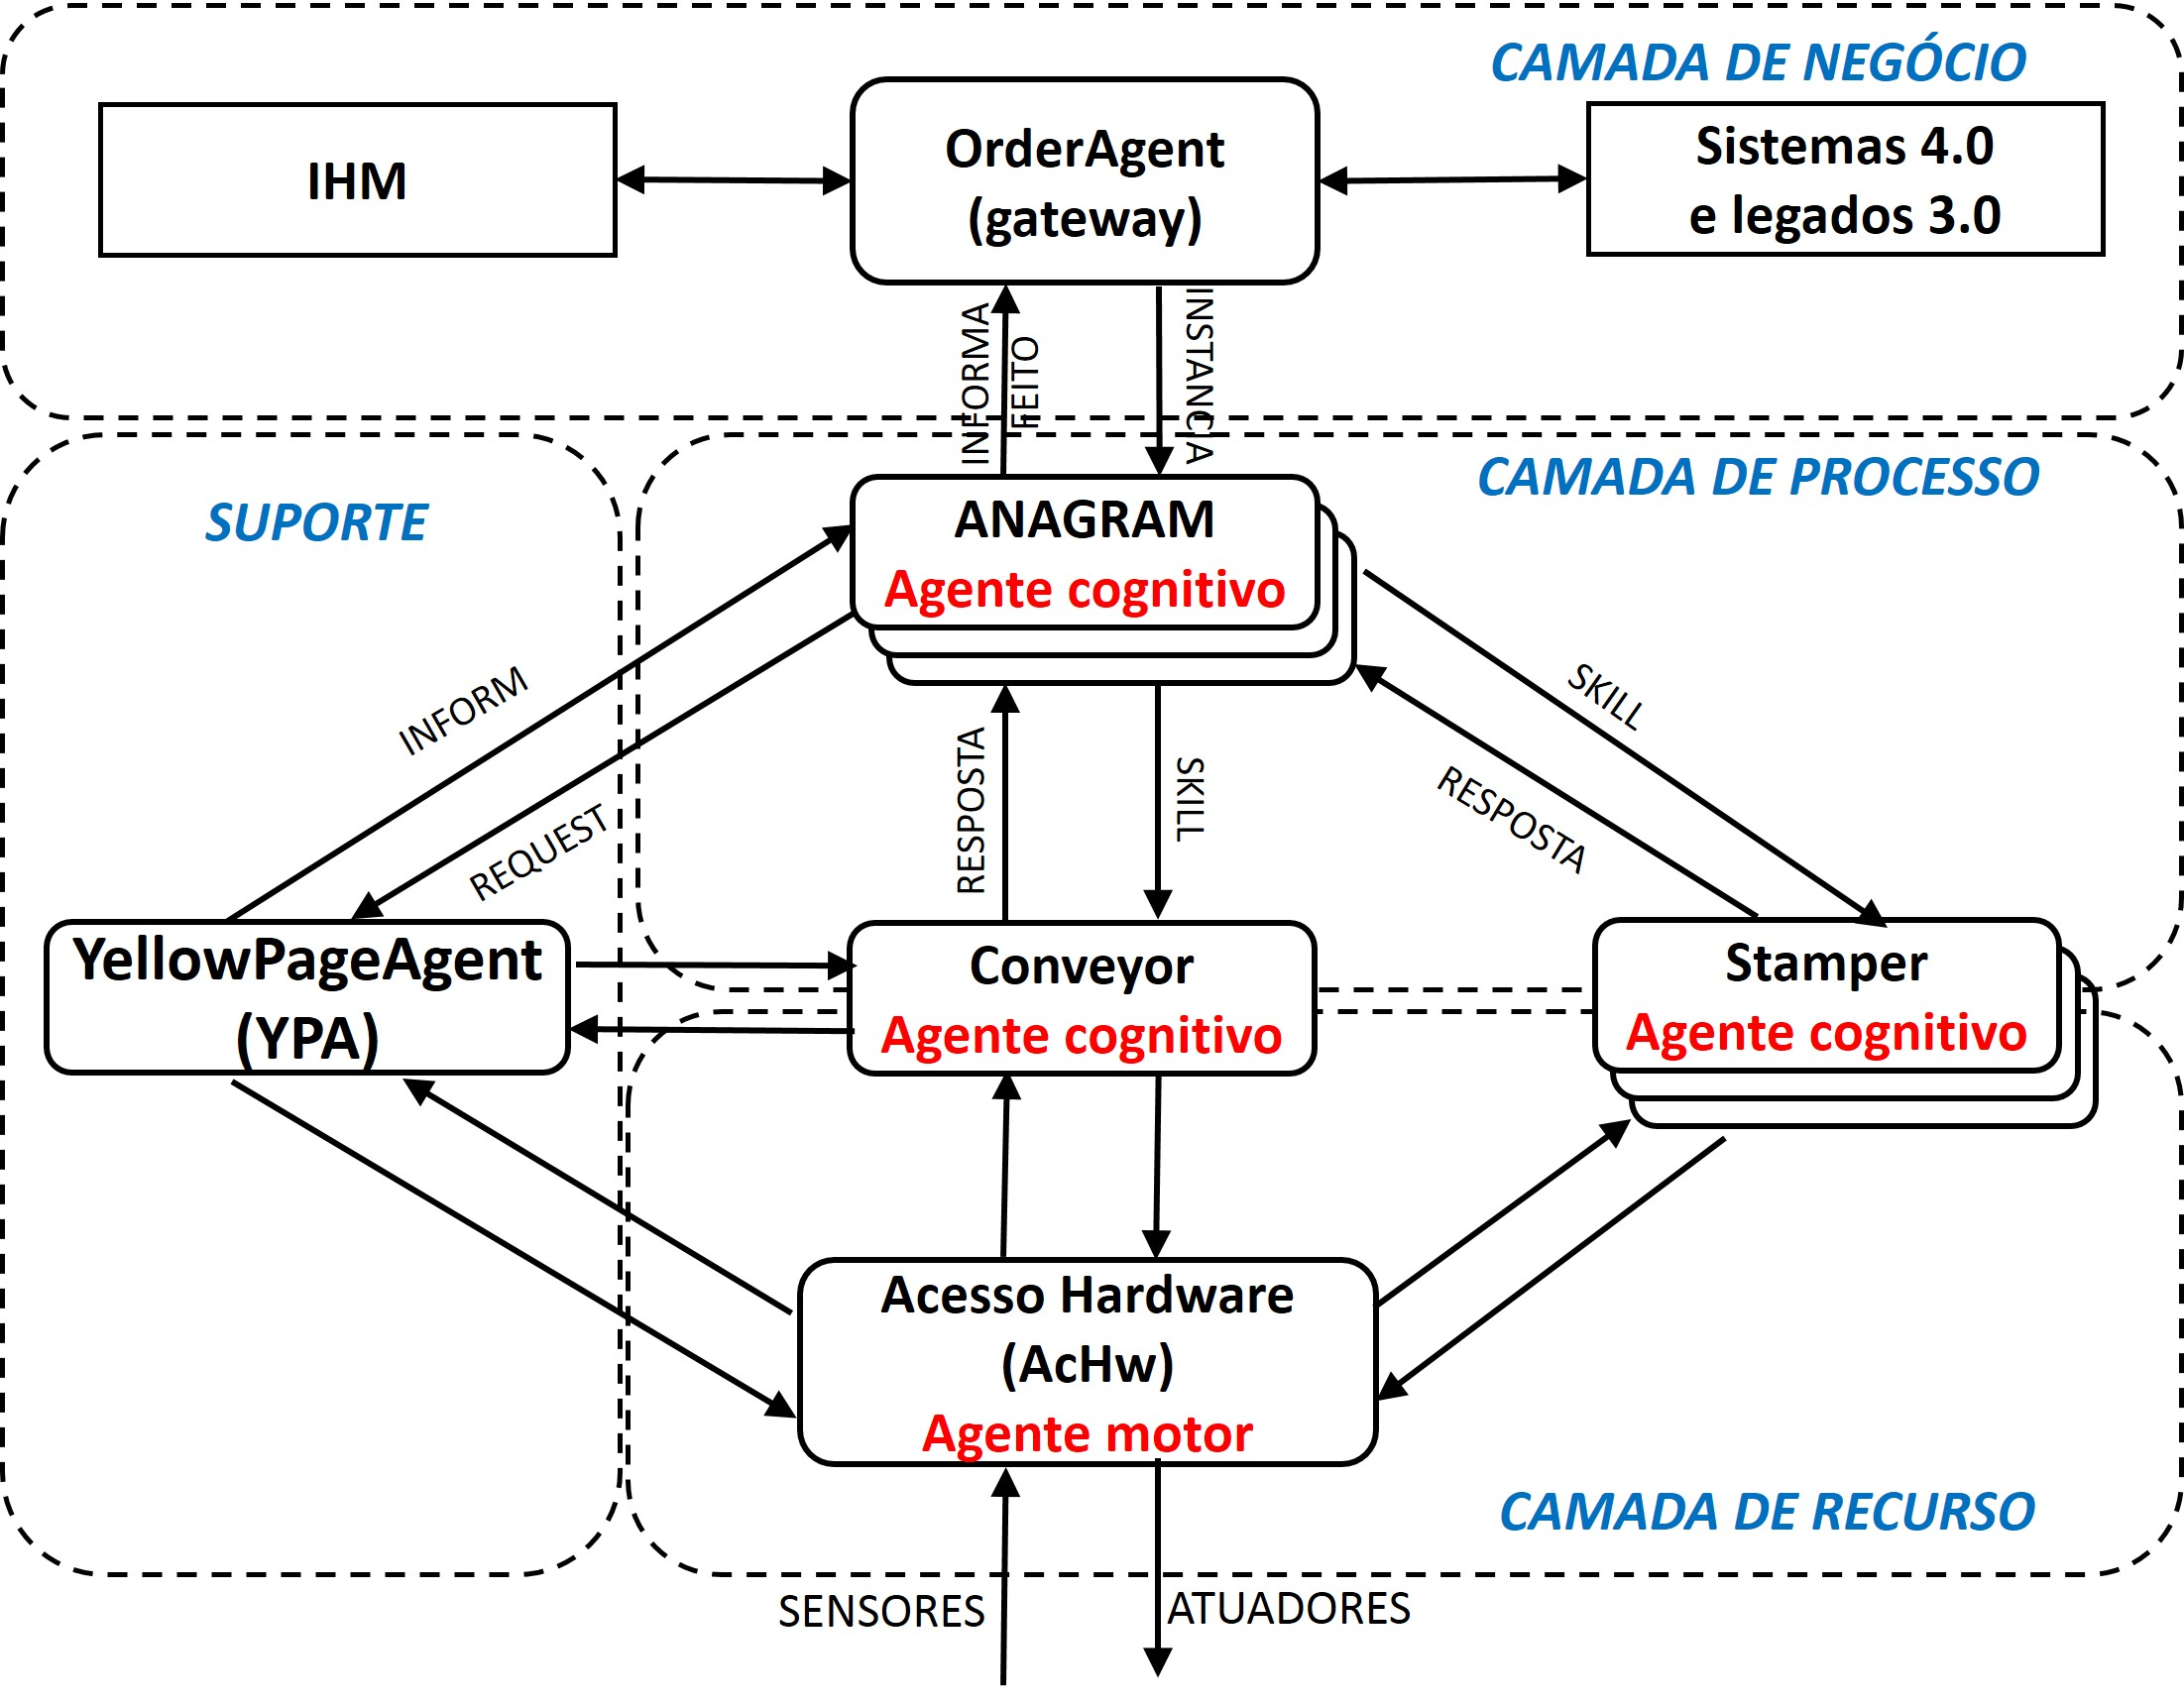
\includegraphics[width=8.9cm, height=7cm]{MeDSE_imagens/F140_SIAPE.jpg}
	\caption{Geração da arquitetura SIAPE com base em EPS}
	%\footnotesize{Fonte: O autor}
	\label{fig:eps_arquitetura_1}
\end{figure}

A Figura \ref{fig:eps_arquitetura_1} ilustra a arquitetura do SIAPE que foi baseada na arquitetura de Cavalcante para um sistema de montagem. Na figura os recursos são agentes cognitivos ou agentes motores que realizam as operações do processo de montagem diretamente nos sensores e atuadores do sistema. \par 
O agente AcHw do SIAPE  tem a principal função de identificar, em tempo real, os módulos que estão presentes no  sistema e informá-los ao agente  \textit{YPA}. Uma vez identificados no \textit{YPA}, os demais agentes tem acesso aos \textit{skills} do AcHW, notadamente o agente Anagram, que usa essas informações para realizar o processo produtivo. 

O agente \textit{OrderAgent} instancia agentes Anagram (agente Produto na arquitetura) que conhece todas as etapas de produção que envolve o agente Stamper e o agente Conveyor. 

O operador pode se comunicar com o sistema por meio da Interface Homem Máquina (IHM) que acessa diretamente o \textit{OrderAgent}. Este também pode ser usado com a função de \textit{gateway} na comunicação tanto de sistema I4.0, isto é, sistemas aderentes à plataforma i4.0, quanto de ambientes I3.0, isto é, sistema flexíveis comuns aos sistemas da 3ª Revolução Industrial.


% SEÇÃO III
\section{EXPERIMENTAÇÃO}	


\subsection{Descrição do Produto UFAM}

O Produto UFAM é um sistema de carimbos de letras para a montagem de anagramas a partir de um CLP e módulos
pneumáticos, tal como os sistemas de montagem atuais, isto é, i3.0.
O Produto UFAM originou a parte de hardware do SIAPE com as devidas melhorias e restrições impostas
pelo cliente. Então, as características do SIAPE são herdadas tanto de ambientes i3.0, quanto de 
ambientes i4.0.
O Produto UFAM é o resultado da integração entre seis subsistemas: um sistema microcontrolado, que utiliza 
entradas analógicas e digitais como entradas e saídas do sistema; um sistema de atuadores, composto por um 
motor DC alimentado com 24V DC, lâmpadas de 24V DC, uma lâmpada de 127V AC, e eletroválvulas de 6bar que são 
controladas por solenóides de 24V DC; um sistema de sensores composto por 6 sensores magnéticos e 1 sensor de 
presença; um sistema de ar comprimido com cinco ramificações de 6 bar. Esses sistemas são alimentados com por 
uma fonte elétrica que fornece 127V DC e 24V DC e tem a sua inicialização dada por um operador humano que liga 
o sistema e insere um palete para que seja processado pelo sistema de manufatura. A Figura \ref{F130} mostra o 
Produto UFAM.


\begin{figure}
	\centering
	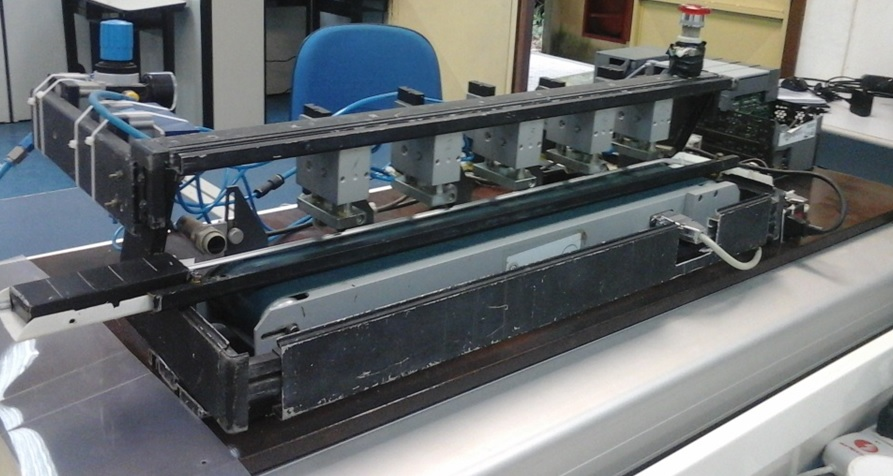
\includegraphics[width=8.9cm, height=5cm]{MeDSE_imagens/F130_PRODUTO_UFAM.jpg} 
	\caption{Produto UFAM}
	\label{F130}
\end{figure}


\subsubsection{Descrição de funcionamento do Produto UFAM}

Para que o sistema seja energizado o operador necessita acionar a chave 1 (CH1: on-off) para a 
alimentação da rede 127/220VAC ser aplicada ao sistema elétrico do hardware do Produto UFAM. O 
código Ladder do Produto UFAM está configurado para realizar a energização sequencial das eletroválvulas 
no tempo de 0,5 segundos entre as mesmas. Assim sendo, tem-se como resultado o posicionamento das 
eletroválvulas iniciando por SL1 e finalizado por SL5. O palete, ao ser detectado pelo sensor 0 (S0)
aciona o motor DC que movimenta a esteira conduzindo o bloco na direção do sensor 1 (S1). 
A lâmpada LP6 identifica o status do sensor 0 (S0). O palete, ao ser detectado por S1, interrompe a 
alimentação do motor DC. Neste momento, a alimentação da eletroválvula correspondente a S1 é interrompida 
e o ar comprimido na eletroválvula, pressiona-a sobre o palete estampando a letra M. Após a estampagem, a 
alimentação da eletroválvula e do motor retorna, movendo a eletroválvula para a posição inicial e movimenta 
a esteira para frente.

O palete, agora com a letra M estampada, move-se em direção aos demais sensores que repete a ação de estampagem 
para as demais letras até completar a palavra do UFAM. Ao chegar no fim da esteira, o bloco estampado é captado 
por S6 que interrompe a alimentação do sistema e aciona o sinalizador (LP7) para que o operador retire o produto 
UFAM da esteira e insira um novo palete. O processo então reinicia até que a produção seja atingida. 	  

%))))))))))))))))))))))))))))))))))))))))))))))))))))))))))))))))))))))))



\section{Experimentação}

Esta seção trata da descrição de um experimento com o SIAPE e suas configurações para produção.

\subsection{Configurações do SIAPE}


Dentre os principais objetivos da configuração para a experimentação pode-se se destacar os seguintes:

\begin{description}
	\item [1]possibilitar que todos os dispositivos especificados estejam  funcionando em  rede;
	\item [2]conseguir fazer com os equipamentos estejam interligados para alimentar os circuitos quando necessário;
	\item [3]monitorar as operações de uma forma que o software possa funcionar com o tempo correto;
	\item [4]possibilitar as realizações das habilidades dos agentes  nas operações necessárias à realização do plano.
\end{description}

\subsection{A configuração para a experimentação}

A Figura \ref{F103} ilustra uma visão simplificada  do estudo de caso que será evoluída até que a configuração 
do sistema seja atingida.

\begin{figure}[h]
	\centering
	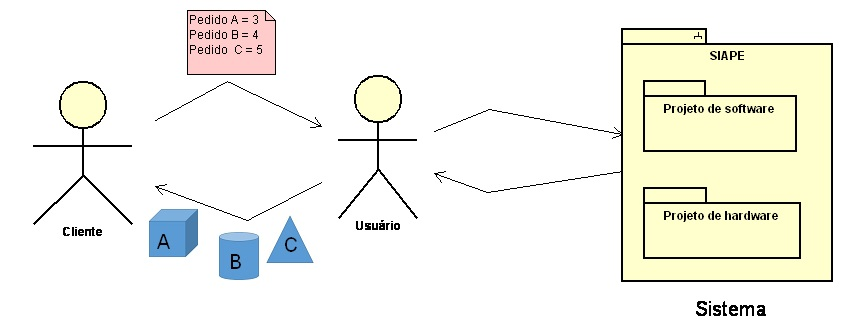
\includegraphics[width=8.9cm, height=6cm]{MeDSE_imagens/F103_SIAPE_ESTUDO_DE_CASO.jpg} 
	\caption{SIAPE - Experimentação}
	\label{F103}
\end{figure}

O estudo de caso é composto por uma solicitação de um cliente. Essa solicitação é composta por três 
pedidos de produção conforme segue:

\begin{description}
	\item[Pedido 1 -] Produto A: A  palavra UFAM; Quantidade = 03 unidades
	\item[Pedido 2 -] Produto  B: A  palavra UTAM; Quantidade = 04 unidades
	\item[Pedido 3 -] Produto  C: A palavra UEA; Quantidade = 05 unidades
\end{description} 

A Realização da  solicitação é processada seguindo os passos a seguir:

\begin{enumerate}
	\item O Cliente solicita os pedidos de produção ao operador.
	\item O Operador insere os pedidos no sistema.
	\item O Sistema realiza os pedidos e retorna os produtos para o operador.
	\item O Operador finalmente atende à solicitação do cliente e entrega os produtos solicitados ao cliente.
\end{enumerate} 

\subsection{Descrições de software e hardware do ambiente de produção.}


O cenário é desenvolvido no ambiente denominado de Ambiente de Produção. A Figura~\ref{F104} ilustra os 
componentes básicos do sistema e suas descrições de hardware e de software são feitas nas tabelas a seguir.

\begin{figure}
	\centering
	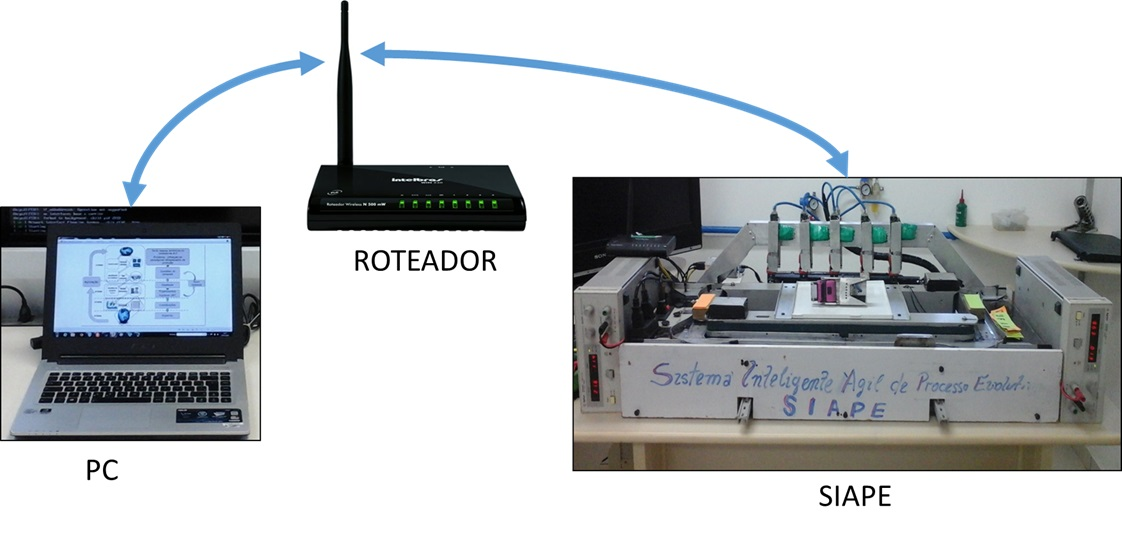
\includegraphics[width=8.9cm, height=8cm]{MeDSE_imagens/F104_SIAPE_AMBIENTE.jpg} 
	\caption{Ambiente de produção para o estudo de caso}
	\label{F104}
\end{figure}


O SIAPE deve ter as características de hardware descritas na Tabela \ref{T6}:

\begin{table}
	\centering
	\caption{SIAPE - Itens características  de hardware}
	\begin{tabular}{|p{4cm}| p{11cm}|l| } \hline
		\textbf{ Item }	   & \textbf{ Descrição}	 \\ \hline
		\textbf{1. M }   & Módulo mecânico\\ \hline
		\textbf{2. E}    & Módulo eletrônico\\ \hline
		\textbf{3.  EEm}  & Entidade eletro-mecânica das letras\\ \hline				
		\textbf{5. EEe}	 & Entidade eletro-mecânica da esteira\\ \hline
	\end{tabular}
	\label{T6}\par
	%	Fonte: Hiram Amaral
\end{table}	


\subsection{Configuração do ambiente de produção.}
Para que o cenário seja realizado no ambiente de produção, este deve ser configurado seguindo os procedimentos relacionados de 1 a 6 que são descritos a seguir e devem ser acompanhados pela ilustração da Figura \ref{F105}.\par 
\begin{figure}[!h]
	\centering
	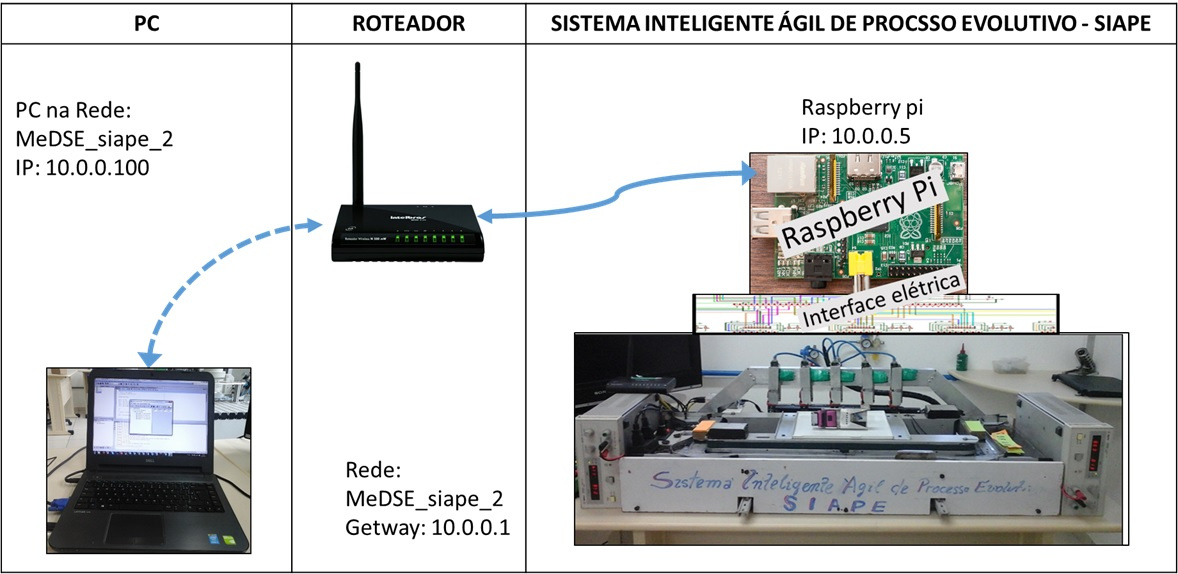
\includegraphics[width=8.9cm, height=7cm]{MeDSE_imagens/F105_SIAPE_ESTUDOD_DE_CASO1.jpg} 
	\caption{Configuração do Ambiente de produção para a experimentação}
	\label{F105}
\end{figure}


%		\begin{description}
\textbf{1.} Ligar o sistema -
Ao ligar a chave \textit{power} do sistema os dispositivos PC, Roteador e SIAPE são energizados e estarão preparados para serem configurados. 

\begin{figure}[!h]
	\centering
	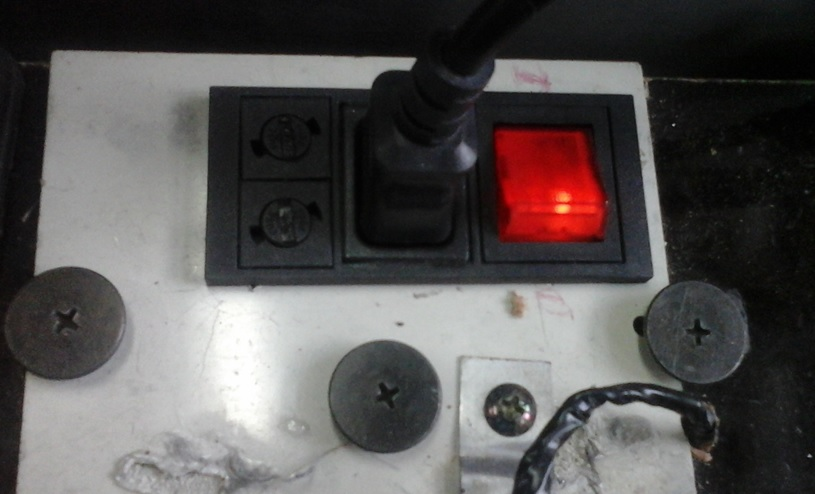
\includegraphics[width=8.9cm, height=5cm]{MeDSE_imagens/F106_SIAPE_POWER.jpg} 
	\caption{Power dos dispositivos}
	\label{F106}
\end{figure}	


\textbf{2.} Configurar o roteador -
Uma rede é estabelecida no roteador com o nome de MeDSE siape com o IP:10.0.0.1. Esta rede será acessada pelo Raspberry Pi e pelos agentes via Protocolos FIPA que são codificados em Java. 

\begin{figure}[!h]
	\centering
	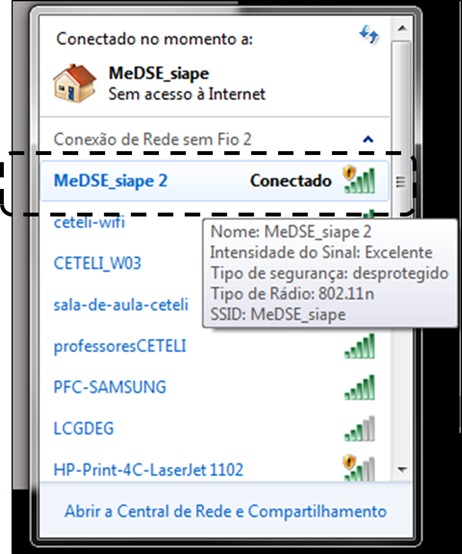
\includegraphics[width=8.9cm, height=5cm]{MeDSE_imagens/F107_SIAPE_MeDSE_siape.jpg} 
	\caption{Rede MeDSE siape - ip:10.0.0.1}
	\label{F107}
\end{figure}

\textbf{3.} Configurar o Raspberry Pi -
O Raspberry Pi é configurado com um IP fixo de número 10.0.0.5 e acessa a Rede MeDSE siape via cabo RJ45. O Raspberry é conectado diretamente à interface elétrica e fornecerá ao agente YPA a informação dos módulos presentes na interface  elétrica;


\begin{figure}[!h]
	\centering
	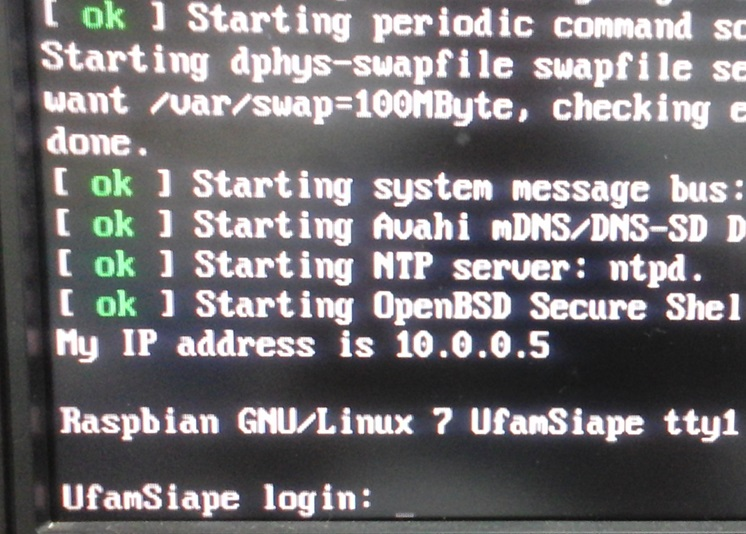
\includegraphics[width=8.9cm, height=4cm]{MeDSE_imagens/F108_SIAPE_RPI.jpg} 
	\caption{Rede MeDSE siape - Raspberry Pi - 10.0.0.5}
	\label{F108}
\end{figure}


\textbf{4.} Criar uma plataforma Jade -
No PC acessar o IDE Netbeans e criar uma plataforma Jade, dentro do main container criar um agente YPA. Essas ações são conseguidas por meio codificação Java no arquivo mainsiape.java;

\begin{figure}[!h]
	\centering
	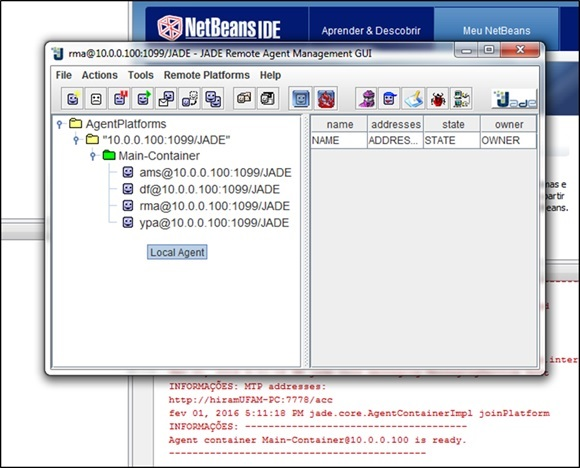
\includegraphics[width=8.9cm, height=6cm]{MeDSE_imagens/F109_SIAPE_YPA.jpg} 
	\caption{Plataforma Jade - Agente YPA}
	\label{F109}
\end{figure}


\textbf{5.} Criar um agente AcHw -
Ainda dentro da plataforma Jade, criar um container, e dentro dele criar um agente AcHw. O agente Acesso Hardware é o responsável por fornecer os módulos presentes na interface elétrica ao YPA; 

\begin{figure}[!h]
	\centering
	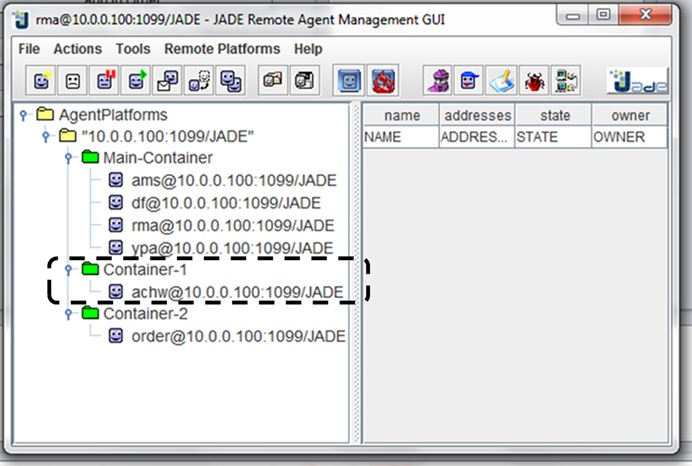
\includegraphics[width=8.9cm, height=5cm]{MeDSE_imagens/F110_SIAPE_AcHw.jpg} 
	\caption{Plataforma Jade -- Agente AcHw}
	\label{F110}
\end{figure}

\textbf{6.} Criar um agente Order.
Criar um segundo container, e dentro desse criar um agente Order. O agente Order é o agente que instancia a interface anagrama responsável em receber as informações do cliente, e depois que receber o plano do agente Order, realizar esse plano.
%		\end{description}

\begin{figure}[!h]
	\centering
	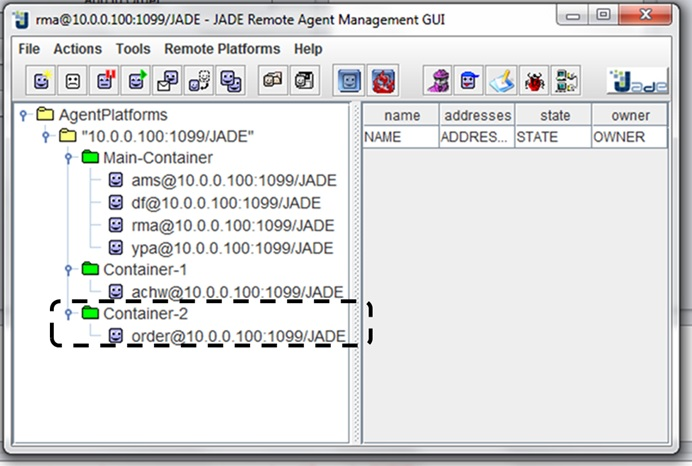
\includegraphics[width=8.9cm, height=5cm]{MeDSE_imagens/F111_SIAPE_ORDER.jpg} 
	\caption{Plataforma Jade - Agente Order}
	\label{F111}
\end{figure}

Quando o agente Order é criado, ele instancia o agente Anagrama que fica acessível ao operador por meio da interface gráfica. O operador deverá inserir os pedidos do cliente na interface, essa atividade inicia o estudo de caso propriamente dito, e este é descrito na próxima seção deste capítulo.




%)))))))))))))))))))))))))))))))))))))))))))))))))))))))))))))))))))))))))))))))))0


% SEÇÃO IV
\section{ANÁLISE DE RESULTADOS E VALIDAÇÃO}


	\section{Realização da experimentação}
	
	
	Nesta seção a experimentação é realizada, isto é, a solicitação do cliente é inserida no sistema pelo operador, 
	o sistema realiza a produção e retorna ao operador os pedidos do cliente na forma de produtos. Esses produtos 
	são entregues ao cliente, atividade que conclui o estudo de caso. Além da realização, os resultados são 
	registrados para que possam ser analisados na próxima seção. \par 
	
	Da mesma forma que foi feito na seção anterior, os procedimentos de 7 a 11 serão realizados e podem ser 
	companhados com as ilustrações de cada atividade e pela ilustração da Figura \ref{F105}.
	
	\textbf{7.} O operador insere os pedidos do clientes na Interface gráfica Anagrama.
	
	O operador segue os procedimento para inserir anagramas na interface gráfica, conforme ilustrado na 
	Figura \ref{F142}. Na ilustração pode-se evidenciar dois pedidos do cliente inseridos na interface 
	gráfica. Note-se que a letra E não está presente no sistema e a palavra UEA não foi inserida no plano 
	de produção. Isso se deve ao fato do sistema não permitir que um recurso inexistente no processo seja 
	utilizado no plano, evitando assim erro do operador.
	\begin{description}
		\item[Pedido 1 -] Produto: A  palavra UFAM; Quantidade = 03 unidades
		\item[Pedido 2 -] Produto: B  palavra UTAM; Quantidade = 04 unidades
	\end{description} 
	
	\begin{figure}[!h]
		\centering
		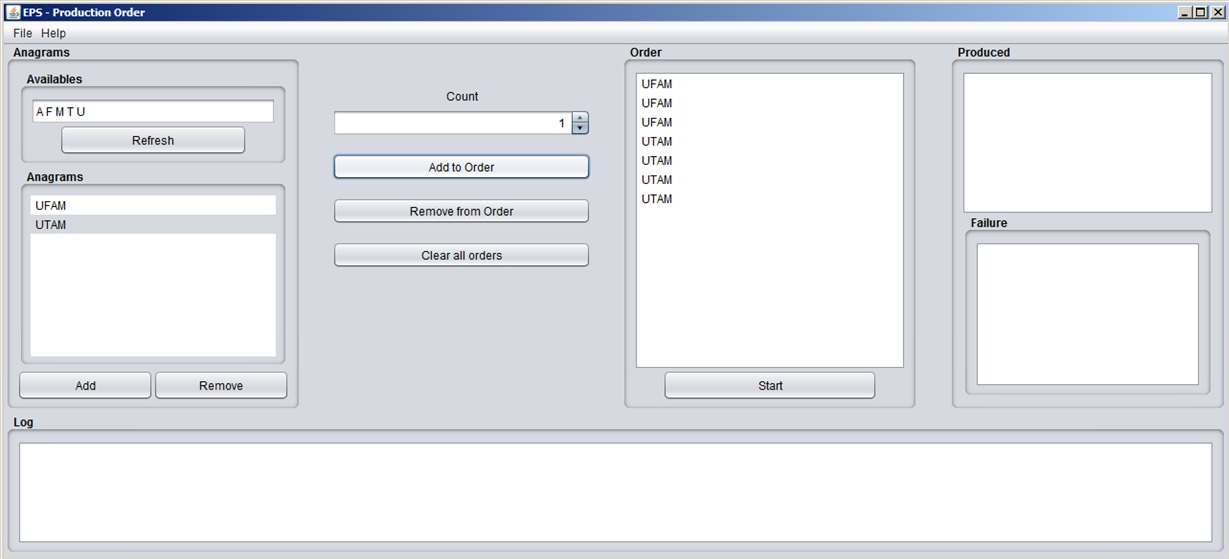
\includegraphics[width=8.9cm, height=6cm]{MeDSE_imagens/F142_PLANO1.jpg} 
		\caption{Plano de produção montado}
		\label{F142}
	\end{figure}
	
	
	\textbf{8.} - O operador inicia o plano de produção.
	
	No momento em que o operador inicia o plano de produção, o agente Anagram extende do agente Produto as 
	informações para a realização de um produto, neste caso, a palavra UFAM. A Figura\ref{F147} ilustra um 
	trecho do código. 
	
	
	\begin{figure}[!h]
		\centering
		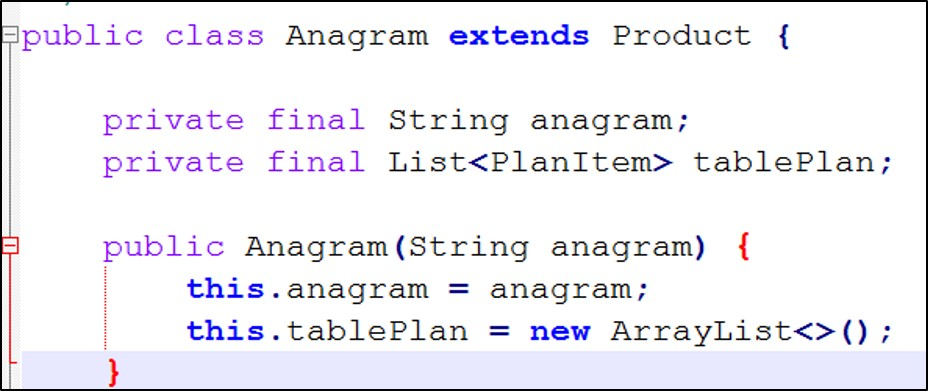
\includegraphics[width=8.9cm, height=4.5cm]{MeDSE_imagens/F147_extends.jpg} 
		\caption{SIAPE: trecho extends}
		\label{F147}
	\end{figure}
	
	Neste momento o agente Produto instancia o agente Anagram com os parâmetros necessários à produção da
	palavra UFAM e o seguinte método é realizado:
	
	1) É definido o agente AcHw com os parâmetros que deverão ser configurados para realizar a produção 
	conforme ilustrado na Figura \ref{F148}:
	
	\begin{figure}[!h]
		\centering
		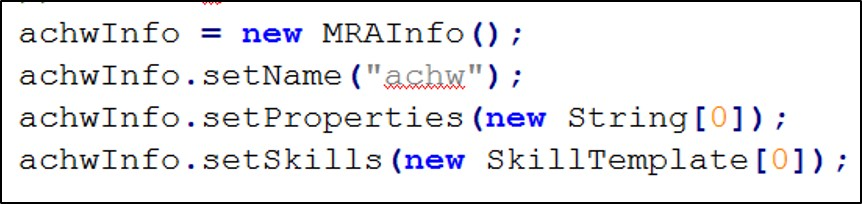
\includegraphics[width=8.9cm, height=2.5cm]{MeDSE_imagens/F148_achw.jpg} 
		\caption{SIAPE: trecho achw}
		\label{F148}
	\end{figure}
	
	2) As letras disponíveis no sistemas ficam acessíveis para ser utilizadas no processo de montagem de 
	acordo com as solicitações do operador. A Figura \ref{F149} ilustra o trecho desse código.
	
	\begin{figure}[!h]
		\centering
		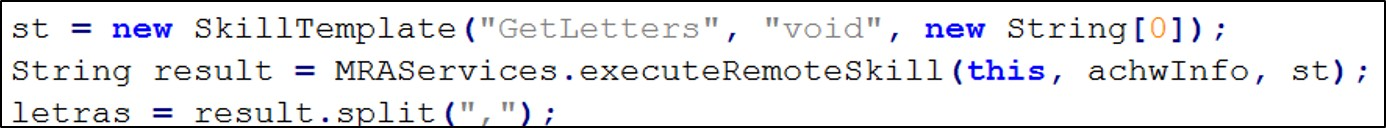
\includegraphics[width=8.9cm, height=2cm]{MeDSE_imagens/F149_letters.jpg} 
		\caption{SIAPE: trecho GetLetters}
		\label{F149}
	\end{figure}
	
	3) A Figura \ref{F150} ilustra o plano de produção que é criado utilizando-se as letras disponíveis 
	que são organizadas conforme a sequência, primeiramente, da posição do módulo e depois, da posição 
	da letra no palete.
	
	\begin{figure}[!h]
		\centering
		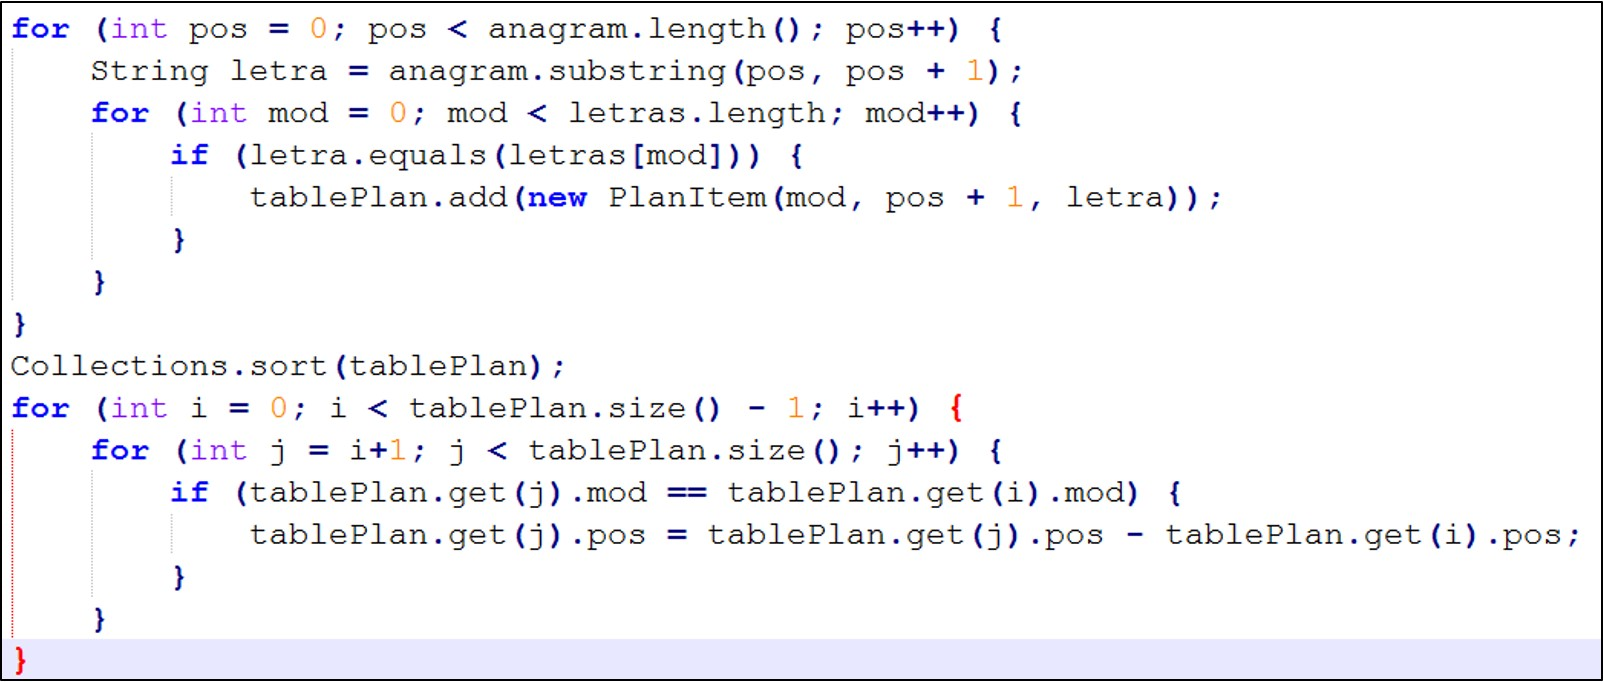
\includegraphics[width=8.9cm, height=7cm]{MeDSE_imagens/F150_criaPlano.jpg} 
		\caption{SIAPE: trecho tablePlan}
		\label{F150}
	\end{figure}
	
	4) Uma vez que as letras são organizada o plano é executado por meio dos skills MoveToStart do agente 
	AcHw. Esse trecho do código está ilustrado na Figura \ref{F151}:
	
	\begin{figure}[!h]
		\centering
		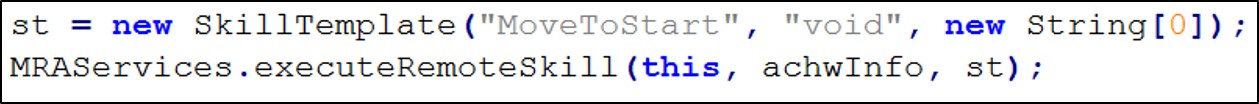
\includegraphics[width=8.9cm, height=1cm]{MeDSE_imagens/F151_MoveTo.jpg} 
		\caption{SIAPE: trecho MoveToStart}
		\label{F151}
	\end{figure}
	5)O palete é movido até o módulo do sistema especificado para a posição definida no palete. Esse método 
	é repetido até que a produção da palavra definida seja concluída, no caso do exemplo do experimento, a 
	palavra UFAM. A Figura \ref{F152} ilustra o trecho do código.
	
	\begin{figure}[!h]
		\centering
		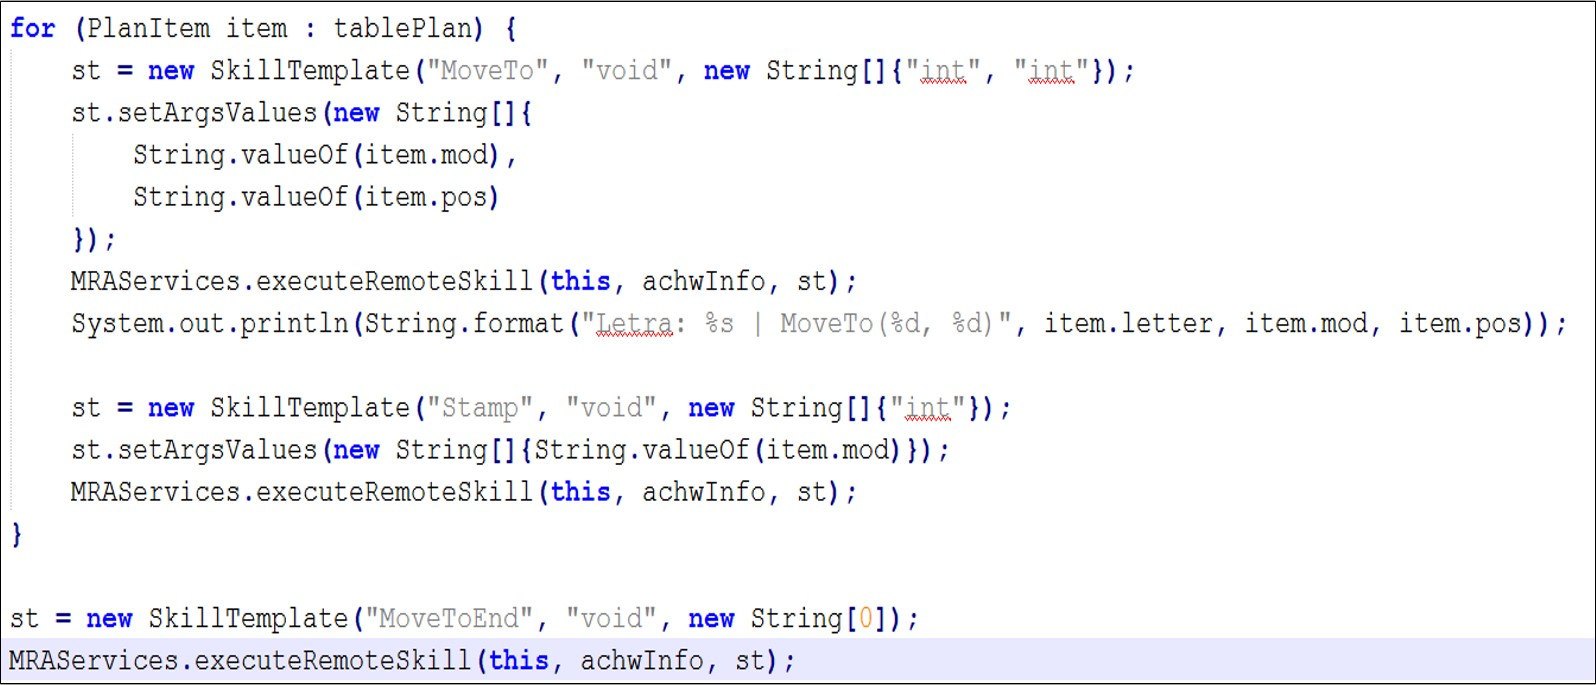
\includegraphics[width=8.9cm, height=7cm]{MeDSE_imagens/F152_MoveToEnd.jpg} 
		\caption{SIAPE: trecho MoveToEnd}
		\label{F152}
	\end{figure}
	
	6) Após realização da produção a situação da produção é informada na tela -- conforme Figura 
	\ref{F153} -- o resultado é mostrado no tela:
	
	\begin{figure}[!h]
		\centering
		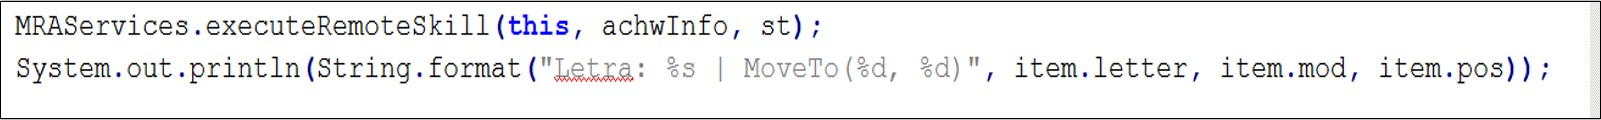
\includegraphics[width=8.9cm, height=2cm]{MeDSE_imagens/F153_PrintStatus.jpg} 
		\caption{SIAPE: trecho Status}
		\label{F153}
	\end{figure}
	
	A Figura \ref{F146} mostra um instantâneo da finalização da produção da palavra UFAM e início da palavra
	UTAM. Note-se que a diferença entre as duas palavras é a letra que se encontra na segunda posição do 
	palete, ou seja, para a letra F, têm-se o seguinte skill MoveTo(1,2), indicando a atuação do módulo 1 
	(letra F) na posição 2 do palete. Para a letra T, têm-se o seguinte skill MoveTo(3,2), indicando a 
	atuação do módulo 3 (letra T) na posição 2 do palete.
	
	\begin{figure}[!h]
		\centering
		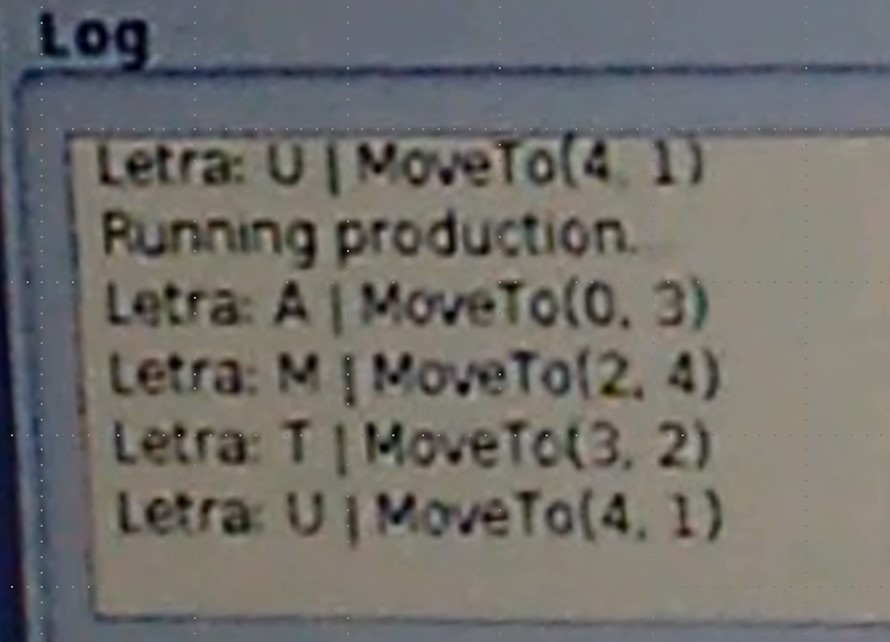
\includegraphics[width=8.9cm, height=4cm]{MeDSE_imagens/F146_LOG.jpg} 
		\caption{Log passagem UFAM para UTAM}
		\label{F146}
	\end{figure}
	
	
	Do ponto de vista do operador quando a tecla \textit{start} é pressionada o plano começa a ser produzido
	obedecendo a sequência definida no plano de produção. Na Figura \ref{F113} pode ser evidenciado que os 
	dois primeiros lotes de produção, relativos aos pedidos A e B já foram produzidos e o terceiro lote será 
	o próximo a ser produzido. Note-se que os produtos A e B usam recursos diferentes (letras T e F) e, nem 
	por isso, houve a necessidade de se parar o sistema para que o recurso fosse trocado de posição. Importante 
	também notar que as quantidades dos produtos também são diferentes (A=3 e B=4) e não houve qualquer parada
	para a alteração da quantidade, isto é, tanto o tipo de recurso quanto a quantidade dos lotes foram alterados 
	em tempo real durante a produção dos produtos A e B.\par 
	O instantâneo mostrado na Figura \ref{F113} também registrou a presença do recurso E (letra E). Isso se 
	deve ao procedimento do operador trocar o módulo da letra T pelo módulo da letra E e atualizar o sistema 
	sem ter que desligar  sistema. Uma vez atualizado, o módulo foi imediatamente incluído no plano de produção
	e realizado no processo de produção.  
	
	\begin{description}
		\item[Pedido 3 -] Produto: C  palavra UEA; Quantidade = 05 unidades
	\end{description} 
	
	\begin{figure}[!h]
		\centering
		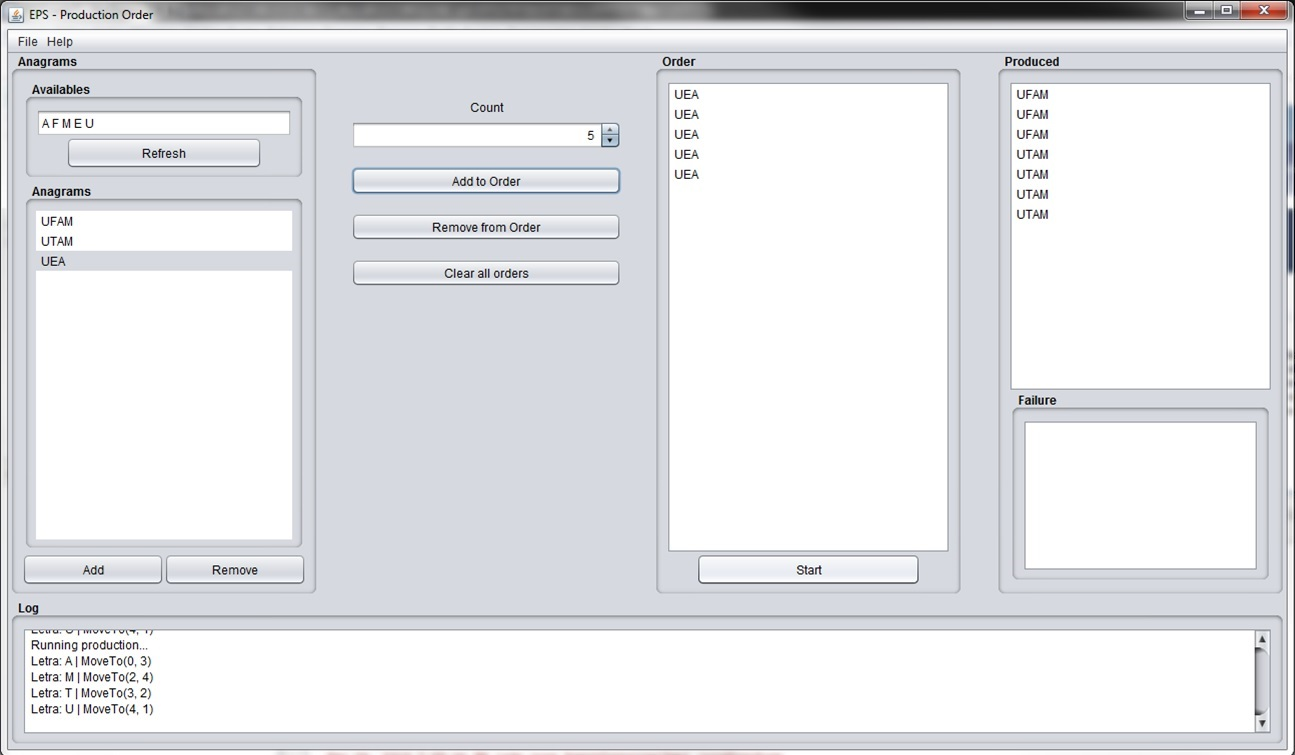
\includegraphics[width=8.9cm, height=8cm]{MeDSE_imagens/F113_SIAPE_PLANO_2_3.jpg} 
		\caption{Realizando Plano de produção}
		\label{F113}
	\end{figure}
	
	Um olhar mais atento às Figuras \ref{F142} e \ref{F113} e às operações realizadas, percebe-se a 
	realização do conceito \textit{plug and produce} pois o tempo necessário para realizar a troca 
	de módulos entre os produtos B e C, a atualização e a inserção do produto C no plano de produção 
	foi em média de 42,25 segundos, que na prática, esta operação representa a troca de um produto 
	com o sistema em funcionamento sendo praticamente nula comparada aos tempos praticados hoje em 
	dia que ficam em torno de 30 a 45 minutos, dependendo do número de recursos que compõem  produto. 
	É claro que há de se considerar o nível reduzido da experimentação realizada, contudo, como as 
	operações realizadas foram possibilitadas devido às características do sistema que são dinâmicas, 
	esses ganhos tendem a se repetir em plantas reais, pois a dinâmica que reconhece e atualiza o 
	sistema se dá no nível de software.\par 
	Outro detalhe importante a ser notado é que o sistema não permite que um recurso (letra) seja 
	inserido no plano sem que o mesmo esteja presente no sistema. Caso ocorra uma falha, como, por 
	exemplo, a retirada de um módulo durante o processo produtivo, o erro é identificado e o sistema 
	não permite que o produto seja produzido. Para que o sistema continue, o recurso pode ser reinserido 
	para que a produção do produto continue.\par    
	
	
	\textbf{9.} O operador recebe a confirmação da realização do plano. Por meio da Figura \ref{F114} 
	pode-se evidenciar que o plano foi totalmente realizado sem nenhuma falha. Note-se que o campo 
	failure está vazio, indicando que que a performance do sistema nesse plano foi 100\%.
	
	
	\begin{figure}[!h]
		\centering
		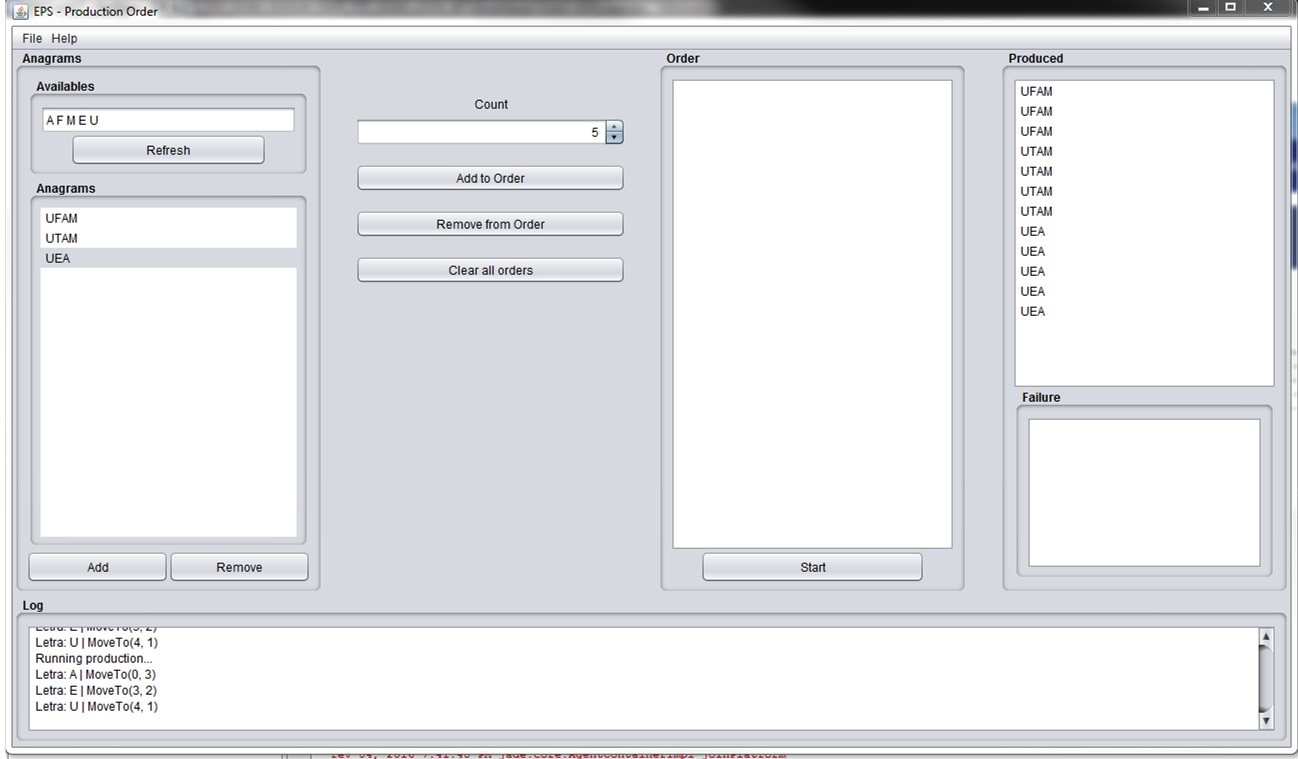
\includegraphics[width=8.9cm, height=8cm]{MeDSE_imagens/F114_SIAPE_PLANO_3_3.jpg} 
		\caption{Interface gráfica com Plano de produção}
		\label{F114}
	\end{figure}
	
	
	\textbf{10.} O operador entrega os produtos e desliga o sistema. 
	
	
	Após a confirmação da realização da experimentação de produção no SIAPE, o operador desliga o 
	sistema e separa os lotes para serem entregues conforme os pedidos dos produtos e suas respectivas 
	quantidades. Entregues os lotes a experimentação está concluída.
	
	A próxima seção analisa os resultados registrados nesta seção e discute os processamentos realizados 
	pelos agentes do sistema.
	
	\begin{center}
		
	\end{center}	
	
	A realização da experimentação evidenciou de uma forma simplificada e operacional a funcionalidade do 
	SIAPE, isto é, as funcionalidade que interessam especificamente ao cliente, pois com o sistema, as 
	necessidades do cliente tendem a ser atendidas e os seus problemas solucionados.\par 
	Além de evidenciar as funcionalidades do sistema, foi possível utilizar o manual de instruções e realizar
	os passos necessários para realizar os pedidos solicitados, neste casos, o plano de produção contendo os 
	produtos ilustrados na Figura  \ref{F115}. Nos detalhes, visão dos lotes e a  finalização de um 
	produto.\par
	
	\begin{figure}[!h]
		\centering
		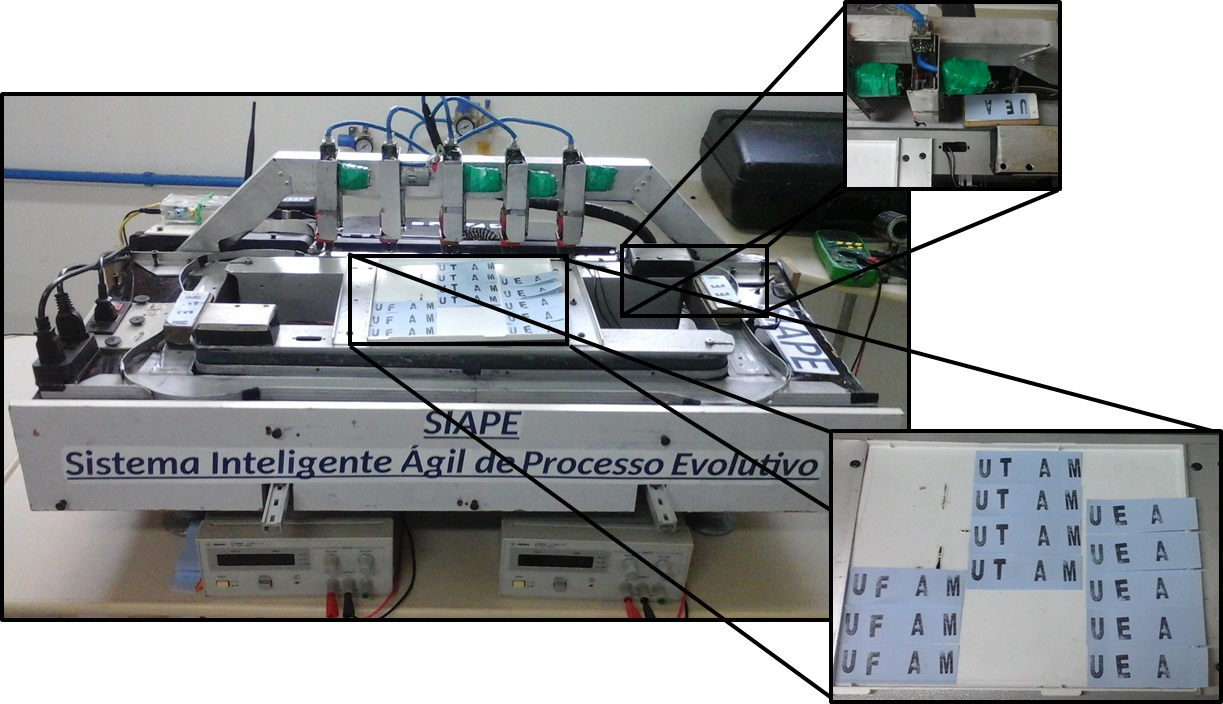
\includegraphics[width=8.9cm, height=8cm]{MeDSE_imagens/F115_SIAPE_Finalizacao_do_Plano_de_Producao.jpg} 
		\caption{Plano de produção realizado}
		\label{F115}
	\end{figure}
	
	Ao final da experimentação o sistema foi ligado, configurado, operado para realizar os produtos. O 
	resultado da produção foi finalmente,   entregue ao cliente. Contudo, existem outras questões que 
	devem ser melhor detalhadas e discutidas como por exemplo:\par 
	1. Como se comportaram os valores temporais e a performance do sistema? \par 
	2. A questão do paradigma evolutivo como potencial solução da customização de massa, ficou evidenciada 
	com a experimentação?\par 
	3. Como ficou a relação entre os referenciais internos e externos e suas  implicações sobre a ciência, 
	a tecnologia e a inovação? \par 
	Essas questões são abordadas no Capítulo 5, a seguir, que analisa os resultados da pesquisa. 
	
	%O sistema foi ligado, configurado, operado para realizar os produtos. O resultado da produção foi 
	finalmente,   entregue ao cliente. Contudo, existem outras questões em níveis mais elevados que devem 
	ser discutidas de uma forma mais detalhada, por exemplo, como se comportaram os valores temporais e a 
	performance do sistema? A questão do paradigma evolutivo como potencial solução da customização de 
	massa, ficou evidenciada com a experimentação? Como ficou a relação entre os referencias internos e 
	externos e suas  implicações sobre a ciência, a tecnologia e a inovação. Essas questões são abordadas 
	no Capítulo 5 que analisa os resultados da pesquisa. 


%==========================================
% SEÇÃO V
\section{Análises de resultados e validação}


\section{Análise de resultados e validação}

O documento de Concepção do Sistema, entregue na Etapa 1 do MeDSE (Capítulo~\ref{cap:desenvolvimento}), 
contém os Requisitos Iniciais e o cenário que foi montado para a realização da experimentação 
(Capítulo~\ref{cap:estudo_de_caso}). A partir dos Requisitos Iniciais, foram processados seguidos 
refinamentos que culminaram na elaboração do projeto de sistema. O projeto de sistema foi transformado 
em simulações que foram transformadas em protótipos, e esses foram testados e validados, modular e 
sistemicamente, contra as especificações técnicas e requisitos. O estudo de caso realizou três pedidos
de clientes. Essa realização produziu os resultados que são analisados neste capítulo.

Duas seções são utilizadas para processar a análise e a validação. Na primeira seção é elaborado um modelo
estático, contudo mais detalhado da produção de um produto usando os recursos do SIAPE. Esse exemplo de 
produção é usado conjuntamente com os resultados da experimentação para evidenciar que as restrições, os
requisitos e as capacidades constantes na Tabela \ref{T14}, foram alcançadas evidenciando a validação do 
SIAPE contra os requisitos propostos.

Na segunda seção esse mesmo modelo é utilizado para evidenciar comparações de performance contra o sistema 
denominado de Produto UFAM que serviu de base para o desenvolvimento do Produto SIAPE. A partir das 
comparações são realizadas algumas discussões em torno dos resultados para concluir a validação do SIAPE 
como um sistema evolutivo.  
%=========================================================================================================	

\begin{table}[!h]
	\centering
	\caption{	SIAPE - REQUISITOS / RESTRIÇÕES /CAPACIDADES		}
	\begin{tabular}{ |c | p{2.5cm}| p{3cm}|c| } \hline
		\textbf{Item} 	   & \textbf{Tipo} &\textbf{ Descrição} & \textbf{Código}\\ \hline
		
		01   & Restrição & tensão DC1 & RS01 \\ \hline
		02   & Restrição & corrente DC & RS02 \\ \hline
		03   & Restrição & Força módulo - elétrica & RS03 \\ \hline
		04   & Cliente-Performance & ciclo de produção mínimo & RQ01 \\ \hline
		05   & Cliente-Performance & setup simplificado  & RQ02 \\ \hline
		06   & Cliente-Performance & ramp up mínimo & RQ03 \\ \hline
		07   & Cliente-Performance &  lead time mínimo& RQ04 \\ \hline
		08   & Cliente-Produto Ufam & carimbar A,F,M,T,U & RQ05 \\ \hline
		09   & Cliente-Produto Ufam & carimbar palavra a partir do RQ5 & RQ06 \\ \hline
		10   & Interno-EPS & modularidade & RQ07 \\ \hline
		11   & Interno-EPS & plugabilidade & RQ08 \\ \hline
		12   & Interno-EPS & reconfigurabilidade & RQ09 \\ \hline
		13   & Enterno-Globalização & Customização & RQ10 \\ \hline
		14   & Externo-Governo & NR-12 (Segurança) & RQ11 \\ \hline
		15   & Externo-Economia & Custos & RQ12 \\ \hline
		16   & Externo-IoT & Plug \& Work & RQ13 \\ \hline
		17   & Externo-i4.o & Integração Horizontal & RQ14 \\ \hline
		18   & Externo-Academia & Estado da arte & RQ15 \\ \hline
	\end{tabular}												
	\label{T14}\par
	%	Fonte: Hiram Amaral
\end{table}
Como forma de organizar a análise a sequência da Tabela \ref{T14} é seguida, e cada tipo de requisito 
é tratado conforme a separação definida a seguir:  

\begin{description}
	\item[Análise de resultado para os requsitos de RQ1 a RQ6 e restrições de RS1 a RS3] -
	Essa análise evidencia o atendimento das necessidades do cliente expressos pelos requisitos RQ1 a RQ6 e 
	restrições RS1 a RS3. Com a expansão da análise consegue-se evidenciar que os objetivos específicos da 
	proposta de pesquisa também foram atendidos. Isso,  quando se  enquadra a realização do sistema  como 
	prova de conceito, tanto do método de desenvolvimento utilizado, quanto da funcionalidade do 
	SIAPE. Considerando essa abordagem, os requisitos RQ1 a RQ6 e as restrições RS01 a RS03 - identificados 
	na Tabela \ref{T14} - são discutidos em maior profundidade.\par
	
	\item[Análise de resultado para os requisitos de RQ7 a RQ12 e capacidades de CP1 a CP3] -
	Aqui, a questão recorrente do problema da customização em massa é tratada pelas principais capacidades 
	dos sistemas evolutivos: capacidade de se adaptar e a capacidade de evoluir. Juntam-se às capacidades, 
	as principais propriedades dos sistemas evolutivos para tratar o problema recorrente da customização 
	de uma forma robusta que proporcione os níveis de competitividades para os produtos produzidos por esses
	tipos de sistemas. Essa análise envolve os requisitos RQ07 a RQ12, conforme descritos na Tabela \ref{T14}.
	
	\item[Análise de resultado para os requisitos de RQ13 a RQ15] -
	Essa análise objetiva evidenciar a relação próxima que tem o estado da arte em paradigmas de produção, 
	aqui considerado o paradigma evolutivo com a fronteira do conhecimento, aqui consideradas a Internet das 
	Coisas e a Indústria 4.0 conforme descrito na Tabela \ref{T14}. 
\end{description} 

Antes de iniciar o processo de análise torna-se necessário relembrar alguns conceitos já mencionados nos 
Capítulos 1 e 2. A Figura \ref{F6} foi refeita convenientemente na horizontal e está ilustrada na
Figura \ref{F118}. Esta figura identifica as fases do ciclo de vida do produto. Relembrando as fases 
do ciclo de vida do produto na fase 1, a equipe de marketing (MKT) realiza pesquisas para identificar 
as demandas não atendidas. Na Fase 2, a Engenharia de Desenvolvimento (END) transforma as necessidades 
não atendidas em produto a ser produzido; a área de Suprimentos (SUP) realiza a compra e a logística 
dos insumos necessários para a realização do produto; a Engenharia de Processo (ENP) na Fase 4, prepara 
o produto para ser aplicado às linhas de produção; a Produção acontece nas linhas de produção - que são 
desenvolvidas a partir de sistemas  de Engenharia e de Computação usando métodos da Automação Industrial 
(foco da análise deste capítulo); a área de Vendas e Distribuição (VDI) realiza as vendas e distribui os 
produtos no Comércio; a área de Instalação e Operações (IOP) realiza a instalação do produto e outras 
operações junto ao cliente;  a Assistência Técnica (ATD) dá suporte ao cliente e ajuda no descarte após 
a finalização do ciclo de vida do produto.  

\begin{figure}[h]
	\centering
	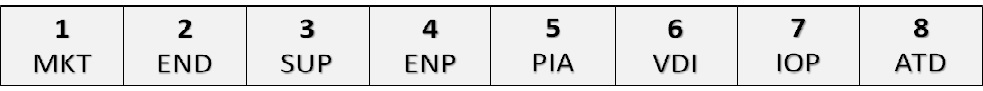
\includegraphics[width=8.9cm, height=1cm]{MeDSE_imagens/F118_CICLO_SIAPE.jpg} 
	\caption{SIAPE - Ciclo de vida do produto}
	\label{F118}
\end{figure}


					
					\section{Análise de resultados das  restrições, requisitos e capacidades}
					
					A partir do ciclo de vida do produto, a fase de produção é explodida para facilitar o entendimento da 
					análise dos resultados. Os componentes do sistema estão identificados, conforme pode ser visualizado 
					na Figura \ref{F120}, foram explicados no Capítulo 2, e são utilizados na análise de cada tipo de 
					requisito nesta subseção.  											
					
					
					\begin{figure}[h]
						\centering
						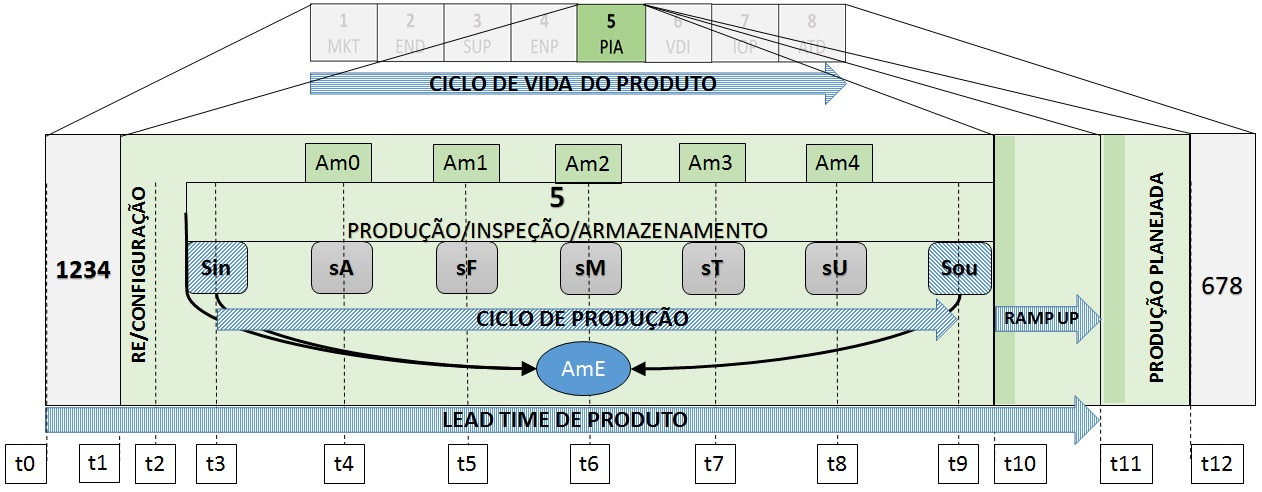
\includegraphics[width=8.9cm, height=6cm]{MeDSE_imagens/F120_SIAPE_CICLO_EXPLODIDO.jpg} 
						\caption{Ciclo de vida do produto: Fase Produção}
						\label{F120}
					\end{figure}
					
					As fases iniciais do ciclo de vida do produto (1234) preparam as atividades da fase de produção, isto é, quando o operador recebe o pedido para ser processado, o SIAPE já está realizado tanto na parte de software quanto na parte de hardware. Essas fases acontecem entre t0 e t1. \par 
					
					É plenamente compreensível para o leitor entender que entre os tempos (ti) podem ou não haver interrupções no processo que aqui não são consideradas.\par 
					
					Quando o operador recebe o pedido de produção, em t1, o SIAPE é configurado e a linha alimentada. Em t2 o operador inicializa a esteira que carrega o palete na direção dos módulos. O agente acesso hardware que monitora os módulos presentes no sistema já tem informado ao OrderAgent todos os módulos do sistema. O OrderAgent por sua vez já incluiu no plano os recursos (letras) solicitadas pelo operador durante a configuração do plano de produção. Caso o recurso faça parte de um dos produtos solicitados, a esteira é movida exatamente para o local do recurso. O Stamper por sua vez realiza seu skill carimbar letra para imprimir a letra sobre o papel que encontra-se no palete. Uma vez carimbada a letra, a esteira é movida para o próximo recurso constante no plano de produção.\par 
					O processo se repete até que o produto esteja totalmente produzido (a palavra completamente impressa no papel)  e o sensor de saída (Sou), no tempo t9,  identifique o palete e registre sua saída do ciclo de produção. De t1 até t9 são percorridas todas as operações de produção necessárias para a realização de uma unidade de produto. De t9 a t10 o produto é armazenado. No período compreendido entre os tempos t10 e t11 encontram-se as atividades relativas à curva de crescimento (ramp up), e de t11 a t12, o período de produção normal, onde todos os recursos de produção estão ajustados e atingiram a produção planejada. As áreas (678) que envolvem a área de Vendas e Distribuição (VDI), a área de Instalação e Operações (IOP) e a Assistência Técnica não são consideradas nestas análises. A Figura   \ref{F120_2} relaciona a Figura \ref{F6} com a Figura \ref{F120} para facilitar o entendimento do conceito de lead time.
					
					
					\begin{figure}[h]
						\centering
						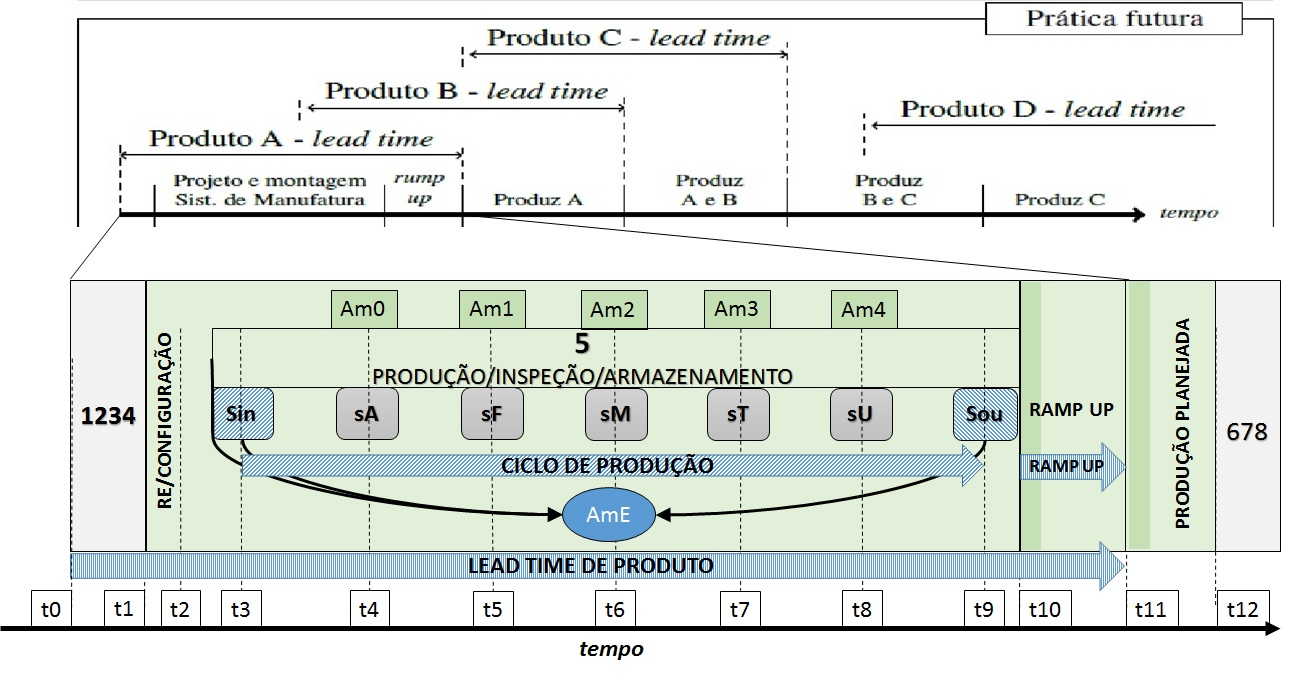
\includegraphics[width=8.9cm, height=6cm]{MeDSE_imagens/F120_2_SIAPE_CICLO_EXPLODIDO.jpg} 
						\caption{Ciclo de vida do produto: Lead time.}
						\label{F120_2}
					\end{figure}
					
					A Figura \ref{F121} ilustra o palete de produção. Quatro posições são codificadas lateralmente no corpo do palete. A localização exata de uma letra é realizada pela posição primeiramente do módulo (Am0 a Am4) e depois pela posição codificada no palete (p1 a p4).
					
					\begin{figure}[h]
						\centering
						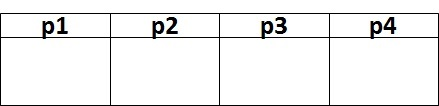
\includegraphics[width=8.9cm, height=1.5cm]{MeDSE_imagens/F121_SIAPE_PALETE.jpg} 
						\caption{SIAPE- Palete}
						\label{F121}
					\end{figure}
					
					O exemplo a seguir produz um anagrama de quatro letras (A, F, M, U) para realizar a palavra UFAM e deve ser acompanhado pela Figura \ref{F123} que ilustra passo-a-passo o processo de produção para uma palavra processando o seguinte \textit{skill}: 
					
					Letra: A | MoveTo(0, 3) | stamp('A')
					Letra: F | MoveTo(1, 2) | stamp('F')
					Letra: M | MoveTo(2, 4) | stamp('M')
					Letra: U | MoveTo(4, 1) | stamp('U')
					
					Para carimbar a letra A:  primeiro o palete é movido:
					\begin{center}
						\textbf{Letra: A | MoveTo(0, 3)}
					\end{center}
					implicando que a esteira levará o palete para a posição (0) que corresponde ao módulo A, e o atuador do módulo A (Am0) carimbará a letra A na posição p3 (3) do palete. 
					
					Essa operação\textbf{(1-Carimba A)}) ocorre no tempo t4, e o processo de detecção - quando necessário - é realizado pelo sensor do módulo A(sA), conforme ilustrado na Figura \ref{F123}
					
					\begin{figure}[!h]
						\centering
						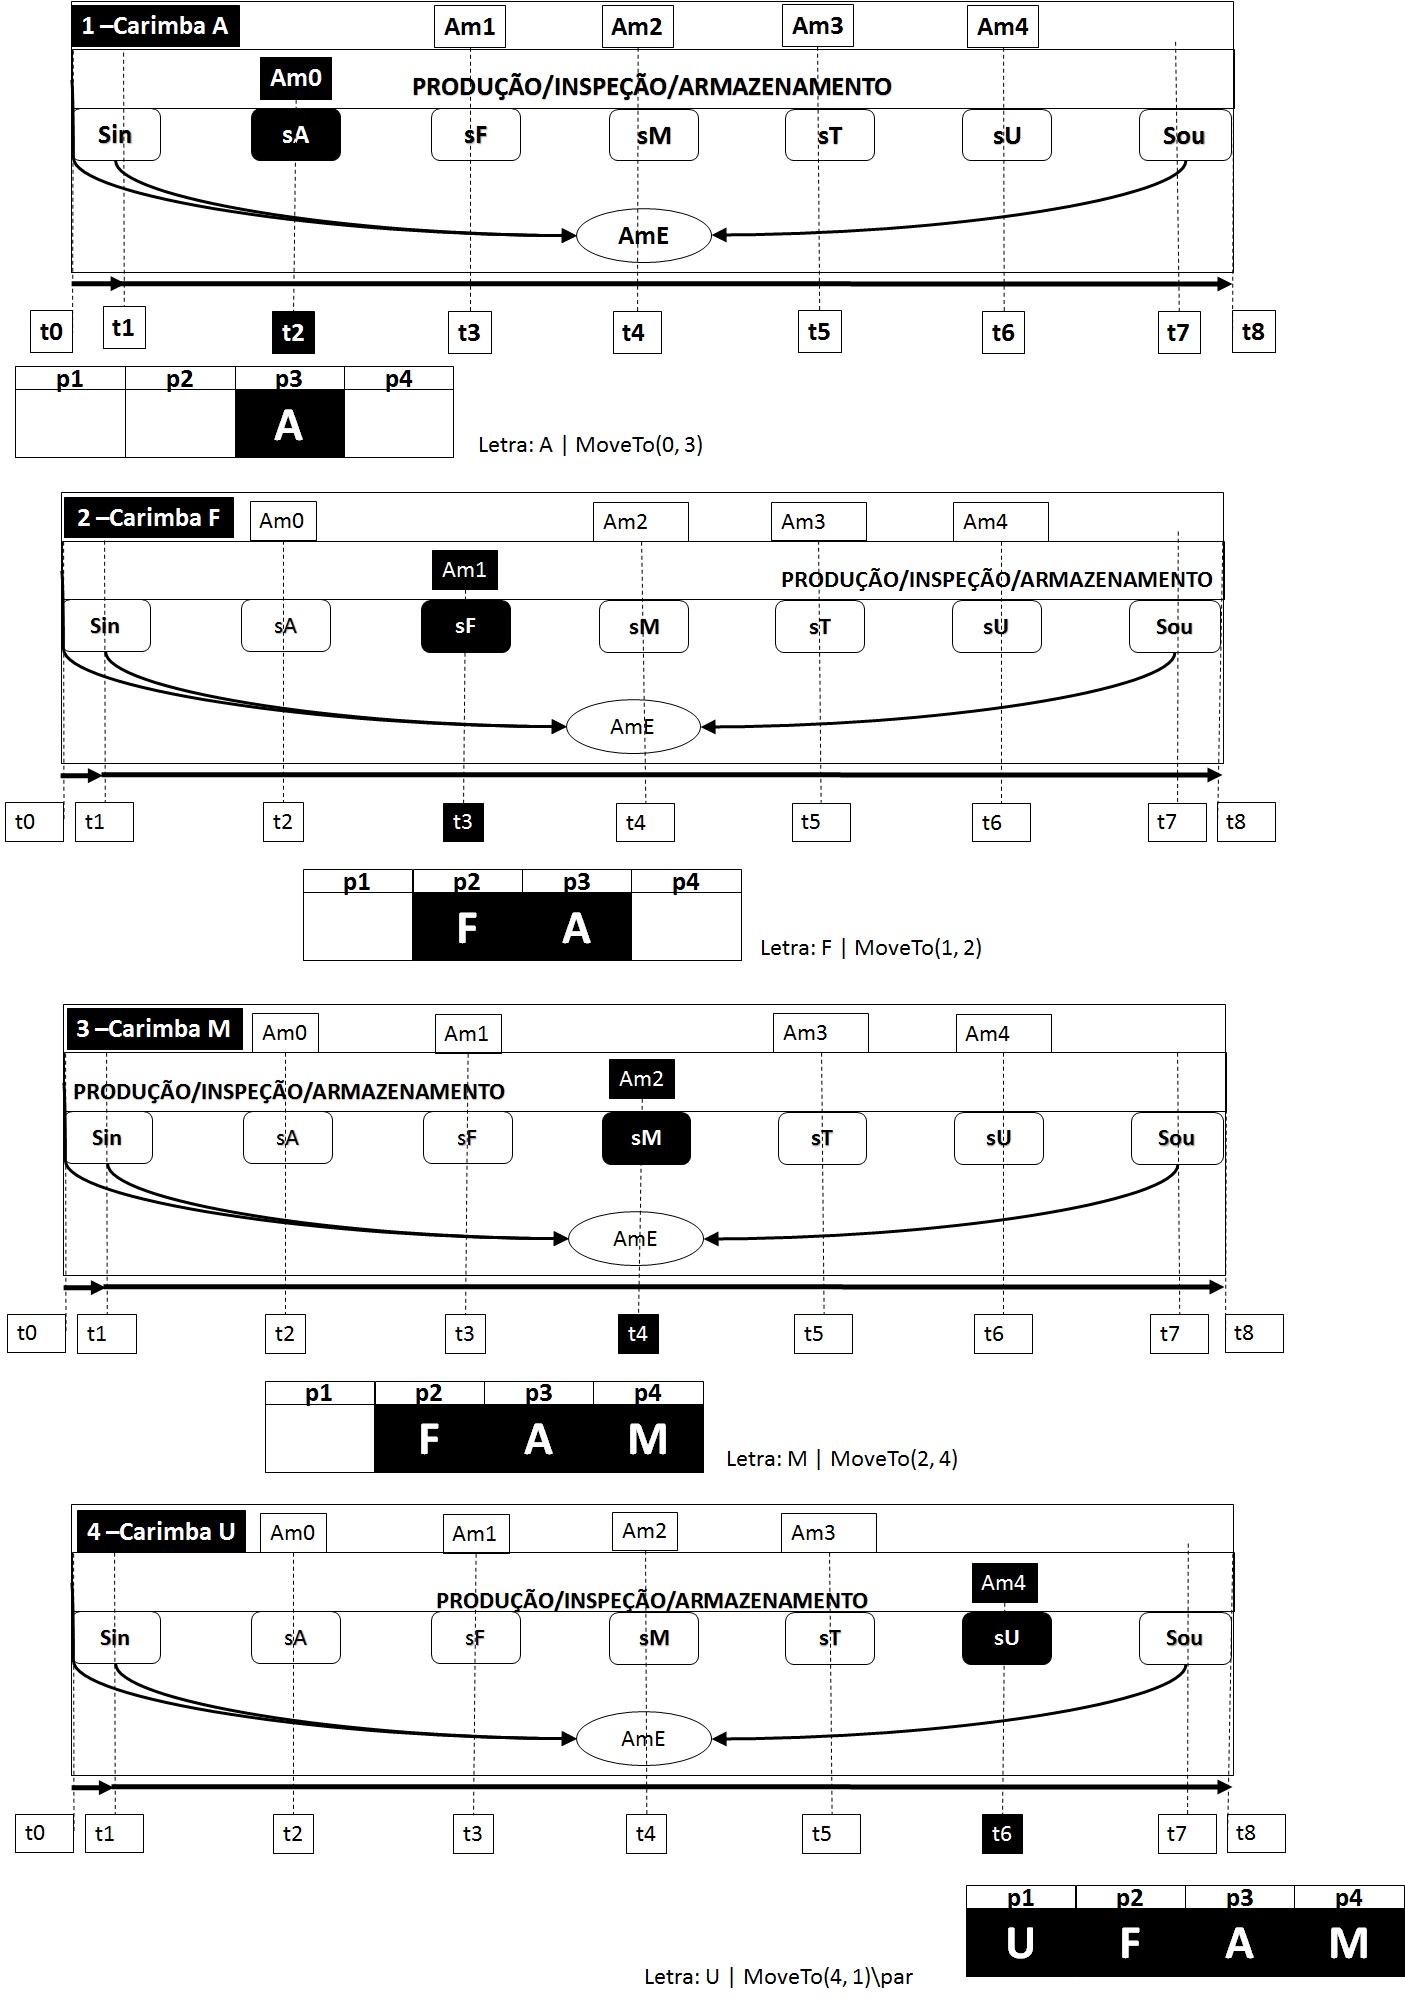
\includegraphics[width=8.9cm, height=22.5cm]{MeDSE_imagens/F123_PALAVRA_UFAM.jpg} 
						\caption{SIAPE- ANAGRAMA UFAM}
						\label{F123}
					\end{figure}
					
					Para carimbar a letra F:  primeiro o palete é movido:
					\begin{center}
						\textbf{Letra: F | MoveTo(1, 2)}
					\end{center}
					implicando que a esteira levará o palete para a posição (1) que corresponde ao módulo F, e o atuador do módulo F (Am1) carimbará a letra F na posição (2) do palete. 
					
					Essa operação \textbf{(2-Carimba F)} ocorre no tempo t5, e o processo de detecção - quando necessário - é realizado pelo sensor do módulo F(sF), conforme ilustrado na Figura \ref{F123}.
					
					
					Para carimbar a letra M: primeiro o palete é movido:
					\begin{center}
						\textbf{Letra: M | MoveTo(2, 4)}
					\end{center}
					implicando que a esteira levará o palete para a posição (2) que corresponde ao módulo M, e o atuador do módulo M (Am2) carimbará a letra M na posição (4) do palete. 
					
					Essa operação \textbf{(3-Carimba M)} ocorre no tempo t6, e o processo de detecção é realizado pelo sensor do módulo M(sM), conforme ilustado na Figura \ref{F123}; 
					
					Para carimbar a letra U. Essa é movida para a seguinte posição
					\begin{center}
						\texttt{Letra: U | MoveTo(1, 2)}
					\end{center}
					implicando que a esteira levará o palete para a posição (4) que corresponde ao módulo U, e o atuador do módulo U (Am4) carimbará a letra U na posição (1) do palete. 
					
					Essa operação \textbf{(4-Carimba U)} ocorre no tempo t8, e o processo de detecção é realizado pelo sensor do módulo U(sU), conforme ilustrado na Figura \ref{F123};
					
					
					\subsection{Análise das restrições de RS1 a RS3}	
					
					O atendimento às restrições impostas pelo cliente no tocante à voltagem (RS1), corrente (RS2) e força (RS3) utilizada pelo SIAPE pode ser evidenciada desde das etapas realizadas na Fase de Realizações do MeDSE, onde os circuitos, componentes e dispositivos utilizados foram especificados e implementados dentro dos limites das restrições, foram registradas no Projeto de Sistema e encontram-se ilustradas nas Figuras \ref{F82} a \ref{F86}. De uma forma geral os circuitos elétricos alimentam o motor DC (esteira) com tensões que podem variar entre de 10 a 24V/2A. No estudo de caso, os módulos das letras foram configurados para trabalharem com 23V DC limitados por uma corrente de 2 A. A Figura \ref{F126} parte A capturou um instantâneo em que um módulo é acionado realizando a tarefa do módulo com uma tensão de 19,9V e um consumo de 1,824A.  O lado B da Figura \ref{F126} registra 12,09V com um consumo de 603 mA no momento em que a esteira carrega o palete na direção dos módulos. Os relés de 24V, o roteador (12V) e o Raspberry Pi (5V) são alimentados com valores menores que os especificados para a esteira e para os módulos. 
					
					\begin{figure}[!h]
						\centering
						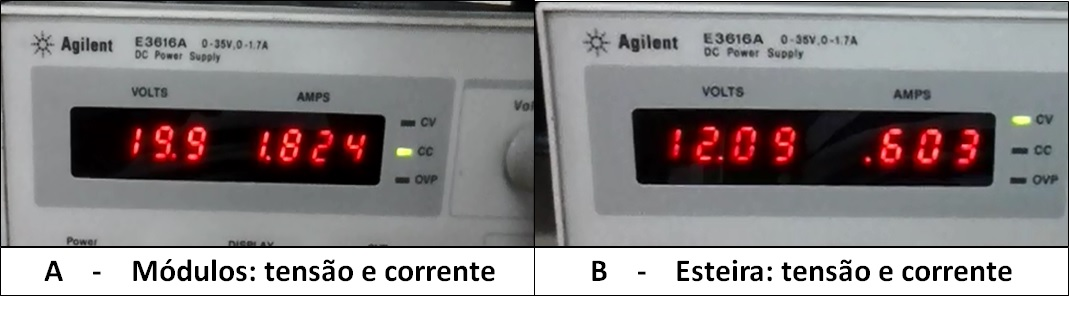
\includegraphics[width=8.9cm, height=3cm]{MeDSE_imagens/F126_SIAPE_TENSAO_CORRENTE.jpg} 
						\caption{SIAPE- Tensão e corrente}
						\label{F126}
					\end{figure}



Para carimbar a letra F:  primeiro o palete é movido:
\begin{center}
	\textbf{Letra: F | MoveTo(1, 2)}
\end{center}
implicando que a esteira levará o palete para a posição (1) que corresponde ao módulo F, e o atuador do módulo F (Am1) carimbará a letra F na posição (2) do palete. 

Essa operação \textbf{(2-Carimba F)} ocorre no tempo t5, e o processo de detecção - quando necessário - é realizado pelo sensor do módulo F(sF), conforme ilustrado na Figura \ref{F123}.


Para carimbar a letra M: primeiro o palete é movido:
\begin{center}
	\textbf{Letra: M | MoveTo(2, 4)}
\end{center}
implicando que a esteira levará o palete para a posição (2) que corresponde ao módulo M, e o atuador do módulo M (Am2) carimbará a letra M na posição (4) do palete. 

Essa operação \textbf{(3-Carimba M)} ocorre no tempo t6, e o processo de detecção é realizado pelo sensor do módulo M(sM), conforme ilustado na Figura \ref{F123}; 

Para carimbar a letra U. Essa é movida para a seguinte posição
\begin{center}
	\texttt{Letra: U | MoveTo(1, 2)}
\end{center}
implicando que a esteira levará o palete para a posição (4) que corresponde ao módulo U, e o atuador do módulo U (Am4) carimbará a letra U na posição (1) do palete. 

Essa operação \textbf{(4-Carimba U)} ocorre no tempo t8, e o processo de detecção é realizado pelo sensor do módulo U(sU), conforme ilustrado na Figura \ref{F123};


\subsection{Análise das restrições de RS1 a RS3}	

O atendimento às restrições impostas pelo cliente no tocante à voltagem (RS1), corrente (RS2) e força (RS3) utilizada pelo SIAPE pode ser evidenciada desde das etapas realizadas na Fase de Realizações do MeDSE, onde os circuitos, componentes e dispositivos utilizados foram especificados e implementados dentro dos limites das restrições, foram registradas no Projeto de Sistema e encontram-se ilustradas nas Figuras \ref{F82} a \ref{F86}. De uma forma geral os circuitos elétricos alimentam o motor DC (esteira) com tensões que podem variar entre de 10 a 24V/2A. No estudo de caso, os módulos das letras foram configurados para trabalharem com 23V DC limitados por uma corrente de 2 A. A Figura \ref{F126} parte A capturou um instantâneo em que um módulo é acionado realizando a tarefa do módulo com uma tensão de 19,9V e um consumo de 1,824A.  O lado B da Figura \ref{F126} registra 12,09V com um consumo de 603 mA no momento em que a esteira carrega o palete na direção dos módulos. Os relés de 24V, o roteador (12V) e o Raspberry Pi (5V) são alimentados com valores menores que os especificados para a esteira e para os módulos. 

\begin{figure}[!h]
	\centering
	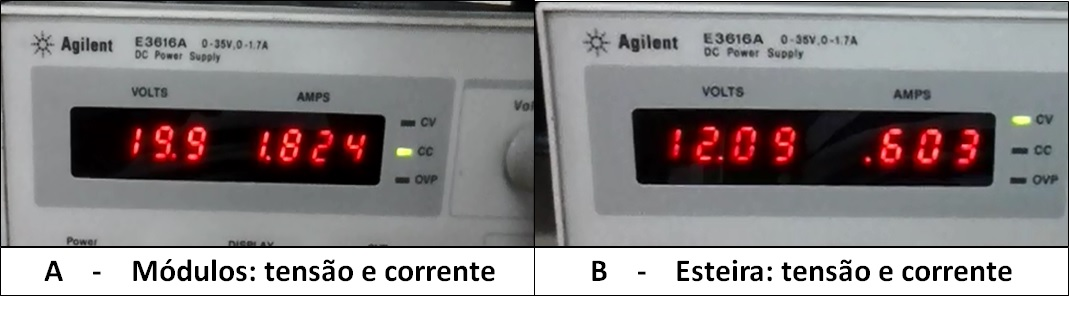
\includegraphics[width=8.9cm, height=3cm]{MeDSE_imagens/F126_SIAPE_TENSAO_CORRENTE.jpg} 
	\caption{SIAPE- Tensão e corrente}
	\label{F126}
\end{figure}

\subsection{Análise e validação dos requisitos RQ1 a RQ6}	

\begin{description}
	\item[Requisito RQ01 - Ciclo de produção:] O ciclo de produção é o tempo gasto nas atividades produtivas para produzir uma unidade de produto. Considerando a ilustração da Figura \ref{F120} o ciclo de produção é realizado entre os tempos t1 a t9, momentos em que a esteira e os atuadores são acionados pelo SIAPE. Nesse momento a esteira é parada e o módulo é acionado para carimbar o papel sobre o palete. O tempo de ciclo de um produto depende das quantidades de operações aplicados em sua produção, isto é o número de letras que são utilizadas para formar uma palavra. Assim para os produtos realizados na experimentação, foram registrados os seguintes tempos de ciclo:
	\begin{enumerate}
		\item Produto A = palavra UFAM: ciclo de 10,53 segundos
		\item Produto B = palavra UTAM:  ciclo de 10,63 segundos 
		\item Produto C = palavra UEA:  ciclo de 10,12 segundos
	\end{enumerate} 
	
	O Produto UFAM realizando os mesmos produtos obteve os seguintes ciclos de produção:
	\begin{enumerate}
		\item Produto A = palavra UFAM: ciclo de 15,42 segundos
		\item Produto B = palavra AFM:  ciclo de 10,55 segundos
		\item Produto C = palavra UTAM: ciclo de 15,33 segundos
	\end{enumerate} 
	
	\item[Requisito RQ02] - setup de produção é o tempo gasto com a configuração ou reconfiguração do sistema do produção. Na Figura \ref{F120}, o setup ocorre entre os tempos t1 e t2. Na experimentação foram produzidos três produtos e realizado dois setups de produção, no início do produto A e entre o produto B e C. Há que se enfatizar que o tempo de setup gasto entre os produtos B e C se deve à realização do conceito do plug and produce. Isso se deve à colaboração entre os agentes inteligentes que processam as alterações de produto e de quantidade entre os produtos A e B em tempo de processamento, não interferindo assim na produção. A Figura \ref{F125} ilustra o ganho reduzido de setup identificado no estudo de caso.
	
	\begin{figure}[h]
		\centering
		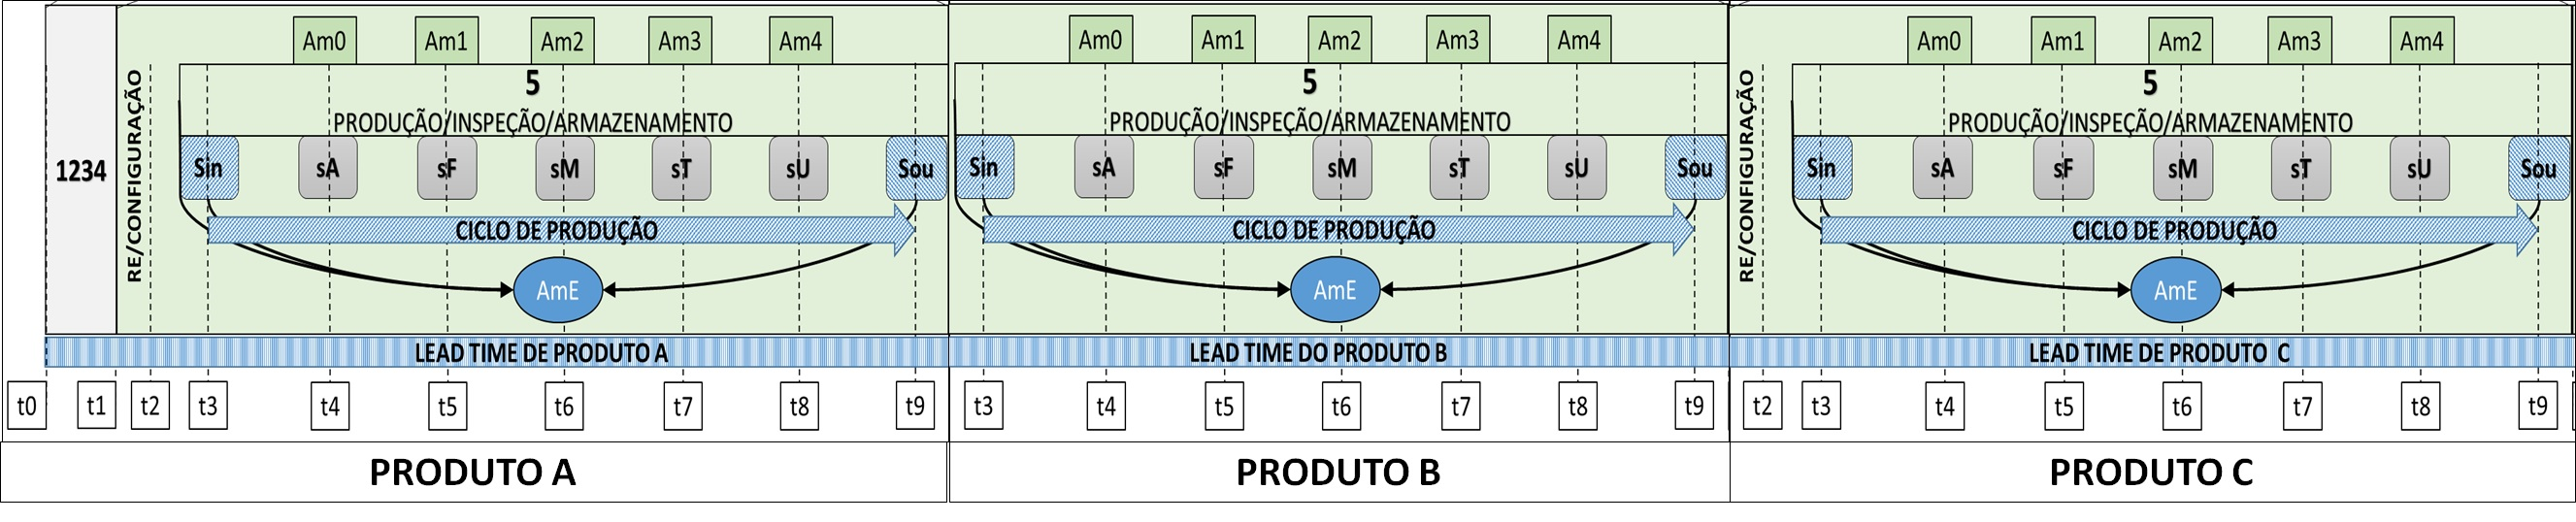
\includegraphics[width=8.9cm, height=5cm]{MeDSE_imagens/F125_SIAPE_CICLO_EXPLODIDOH.jpg} 
		\caption{SIAPE: Setup e Ramp up}
		\label{F125}
	\end{figure}	
	
	\item[Requisito RQ03] - ramp up de produção é o tempo gasto para que os recursos e operações na linha de produção sejam ajustados e se atinja a produção planejada. Na Figura \ref{F120} esse tempo encontra-se entre os tempos t10 e t11.  O SIAPE não gasta tempo com ramp up, pois os recursos do sistema são ajustados durante o tempo de setup para a produção planejada, não necessitando assim, do referido tempo. A eliminação de ramp up também está ilustrada na Figura \ref{F125}.
	
	
	\item[Requisito RQ04] -  Lead time de produto é considerado como o tempo gasto por todas as fases do ciclo de vida do produto  até que se produza uma unidade do produto da produção solicitada pelo cliente. Assim os tempos t0 a t11 cobrem o lead time de produto para este trabalho de pesquisa.  É importante notar que os tempos t11 a t12 cobrem um período em que não há mais desenvolvimento e os recursos e operações estão plenamente ajustadas.	
	
	
	\begin{figure}[h]
		\centering
		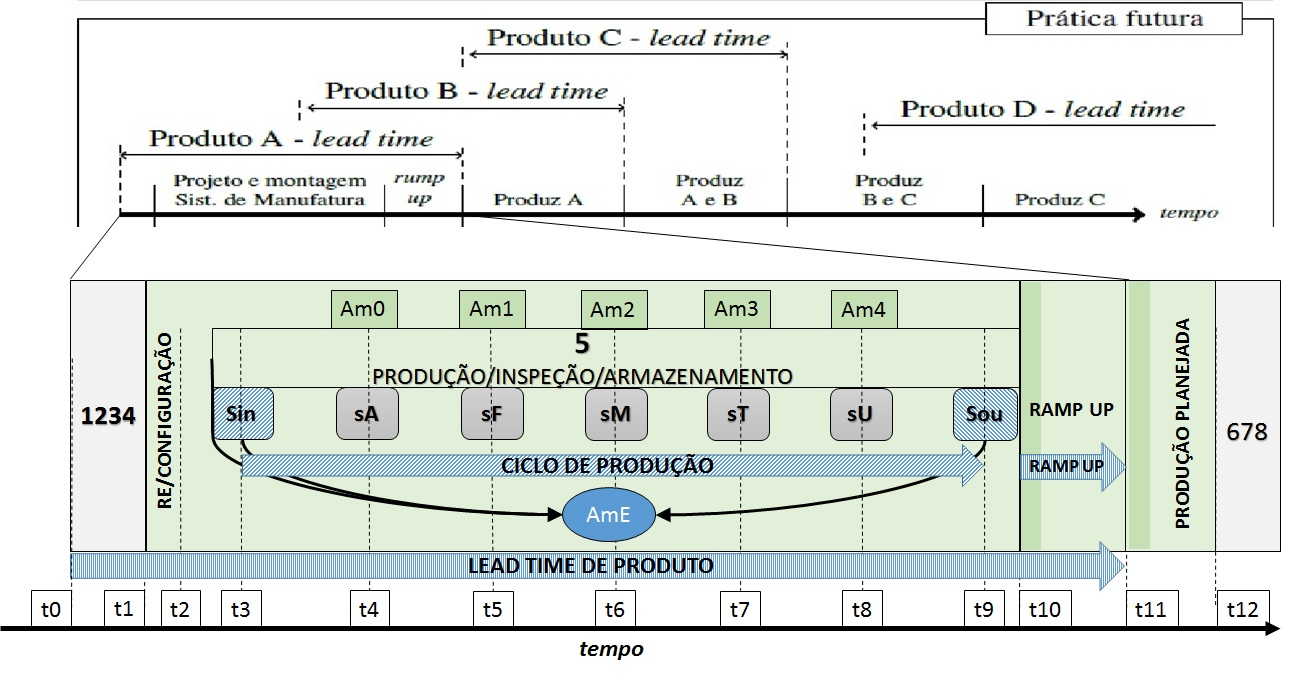
\includegraphics[width=8.9cm, height=10cm]{MeDSE_imagens/F120_2_SIAPE_CICLO_EXPLODIDO.jpg} 
		\caption{SIAPE: Lead time}
		\label{F120_1}
	\end{figure}	
	
	\item[Requisito RQ05] - O quinto requisito especificado pode ser evidenciado por meio da realização tanto do experimento quanto pelo exemplo ilustrado na Figura \ref{F123}.  Os módulos que carimbam as letras A, F, M, T e U foram desenvolvidos para atender esse requisito.\par 
	
	\item[Requisito RQ06] - O sexto requisito especificado pelo cliente determina que palavras sejam originadas das letras disponíveis nos módulos. Mais uma vez é evidente o atendimento desse requisito pelo resultado do estudo de caso. A Figura \ref{F127} ilustra a identificação do módulo com relação à palavra onde o mesmo foi utilizado.
	
	
	\begin{figure}[h]
		\centering
		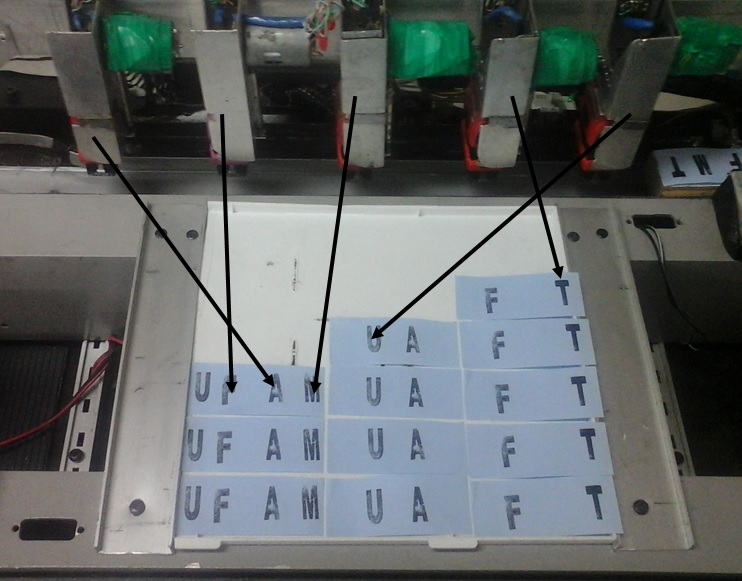
\includegraphics[width=8.9cm, height=5cm]{MeDSE_imagens/F127_SIAPE_AFMTU.jpg} 
		\caption{SIAPE: Anagramas, módulos e palavras}
		\label{F127}
	\end{figure}	
	
	
	
\end{description}					

\subsection{Análise e validação dos requisitos RQ07 a RQ12}	

\begin{description}
	\item[Requisito RQ07] - O requisito modularidade foi tratado desde a fase inicial do método de desenvolvimento MeDSE. Ao se refinar o problema global, em problema regional e depois em problema local tinha como principal objetivo refinar o problema até que ele chegasse ao nível atômico. Uma vez atingido esse nível, os problemas foram modelados, simulados especificados, implementados e validados modularmente, antes dos mesmos serem integrados e validados sistemicamente. É fácil perceber  por meio da verificação, primeiro, da Figura \ref{F13_1} na Fase de Realizações (etapas de 3 a 7) o desenvolvimento dos n módulos necessários para cada tipo de sistema. No caso do SIAPE, foram desenvolvidos cinco módulos para as letras A, F, M, T e U. Segundo, por meio da verificação das Figuras \ref{F69} e \ref{F70} o desenvolvimento dos módulos esteira e carimbador que realizaram a parte hardware do sistema, e na sequencia, a verificação das \ref{F71} a \ref{F74} e \ref{F94} o desenvolvimento dos módulos de software a partir das classes AcHw, YPA, Order, Anagrama e mensagens FIPA até que sejam simuladas. Nas Figuras \ref{F95} e \ref{F96} esses módulos são integrados às suas especificações que realizaram o projeto de sistema e o estudo de caso realiza a funcionalidade do sistema aplicado à produção de três produtos com qualidades e quantidades diferentes. 
	
	
	\item[Requisito RQ08] - A plugabilidade no paradigma EPS é a propriedade que lida com a introdução de novos módulos, enquanto o sistema está em funcionamento. A eficiência do sistema nos tempos t4 a t8 é mantida por meio da reconfiguração dinâmica dos módulos, momento em que o sistema é rapidamente atualizado ao perceber que houve mudanças na disponibilidade de módulos no sistema. No estudo de caso a plugabilidade foi evidenciada na passagem da produção do produto B para o produto C, pois o módulo da letra T - realizou a palavra UTAM - foi conectado após a sua inclusão na interface gráfica. Essa propriedade é melhor detalhada durante a análise do processo que evidencia o conceito plug-and-produce (Plugar e produzir) explicado como uma das capacidades que  o SIAPE tem e que o permite adaptar-se e evoluir com o tempo.
	
	\item[Requisito RQ09] - Uma análise entre os produtos A e B percebe-se que existe uma diferença entre os anagramas UFAM e UTAM que é a letra T no lugar da letra F, implicando que o layout da linha deve ser alterado para que a produção dos anagramas sejam realizados. Contudo, a produção dos dois produtos foi realizada sem que houvesse qualquer interrupção na produção. Isso se deveu à reconfiguração do sistema originada pela negociação entre os agentes no mundo lógico -- conforme mostra a Figura~\ref{F144} -- que foi externada para o mundo real por meio do agente AcHw que atuou diretamente nos atuadores do hardware. Importante também perceber que a negociação foi realizada em paralelo à movimentação do produto A para o produto B, isto é, enquanto a esteira se movia no intervalo entre os produtos A e B, os agentes negociaram, e realizaram a negociação por meio das mensagens FIPA, e promoveram as mudanças necessárias à mudança de produto sem alterar a funcionalidade do sistema.	
	
	\begin{figure}[h]
		\centering
		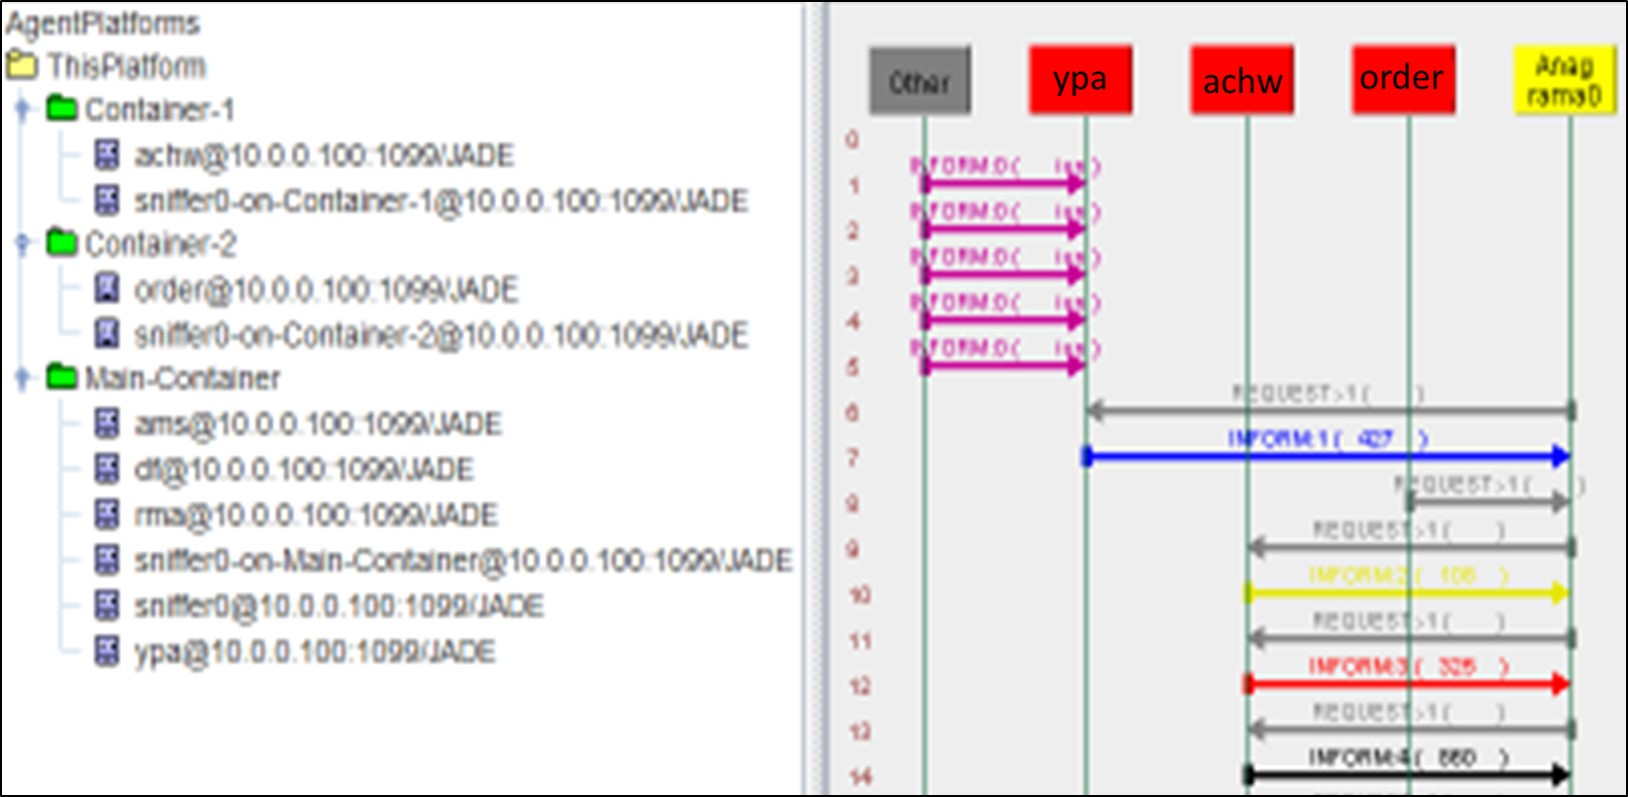
\includegraphics[width=8.9cm, height=5cm]{MeDSE_imagens/F144_ACL.jpg} 
		\caption{SIAPE: Negociação de agentes}
		\label{F144}
	\end{figure}	
	
	
	
	\item[Requisito RQ10] - A customização conforme definida neste trabalho é caracterizada por uma produção variada de produtos com curtos  ciclos de vida. Os lotes de produção são reduzidos para atender às solicitações personalizadas dos clientes. O experimento se enquadra nesse tipo de produção, pois realiza a produção de três produtos diferentes (UFAM, UTAM e UEA) com quantidades diferentes (3,4 e 5). A produção do produto A ocorre dentro dos padrões usuais atuais da indústria, contudo, na passagem do produto A para o produto B já percebe-se diferenças significativas na forma de produzir devido à ausência de reconfiguração e ramp up. Entre o produto e B e C, outra diferença é percebida por haver a inclusão de um módulo no sistema e o tempo gasto com essa operação durar menos de 20\% do tempo normalmente gasto nesse tipo e operação. Isso utilizando  sistema que não são baseados nos sistemas evolutivos, como o exemplo utilizado aqui denominado de Produto UFAM. \par 
	O tratamento realizado no estudo de caso evidencia um potencial promissor em tratar com a questão recorrente da customização de massa. É claro que tanto o tamanho da amostra quanto a própria forma do sistema aqui desenvolvido - em escala reduzida - e a forma e quantidade dos produtos, não favorecem análises mais acuradas, contudo da mesma forma é inegável que os dois sistemas tanto o produto UFAM baseado em ambientes 3.0 quanto o Produto SIAPE baseado no paradigma evolutivo, portanto em sistemas 4.0, são válidos por serem desenvolvidos por um método sistemático de desenvolvimento, o MeDSE, que possibilita a criação de sistemas que podem ser validados e realizados, a exemplo do SIAPE.
	
	\item[Requisito RQ11] - Este requisito foi solicitado para que se evidenciasse a presença do Governo influenciando no desenvolvimento e realização de sistemas de produção no território brasileiro. Assim foram incluídos circuitos que torna o sistema seguro baseado o nas normas NR-12 no item de Segurança no Trabalho em Máquinas e Equipamento que estabelece os procedimentos obrigatórios nos locais destinados a máquinas e equipamentos. Neste item estabelece que as máquinas devem ser equipadas com um ou mais dispositivos de parada de emergência, por meio dos quais possam ser evitadas situações de perigo latentes e existentes. As chaves podem cortar o processamento ao nível de software ou alimentações específicas a nível de hardware. \par 
	A exemplo no nível de hardware a Figura \ref{F128} ilustra alguns trechos de códigos e de partes do esquema elétrico do SIAPE para evidenciar  a atuação da chave SNR--12. A explicação dessa figura deve ser acompanhada com a visualização da Figura \ref{F123}. Na parte inferior (A) da Figura \ref{F128}  a linha de código evidenciada ilustra o comando que aciona a esteira. Quando a chave SRN$-12_1$ está fechada o exemplo ilustrado na Figura \ref{F123} funciona sem interrupção. Considere agora que na passagem do módulo M para o módulo U o operador necessite parar o processo. Ele aciona a chave colocando-a na posição aberta. Na parte de software a informação sai do Raspberry Pi (RPI) e polariza o fotoacoplador (U9) e este, chaveia o transistor Q1, contudo o relé RL1 não consegue ser acionado porque a alimentação de 24V foi interrompida pela RN--12. Quando o operador fechar novamente a chave, o sistema volta a funcionar normalmente e a letra U é carimbada. Isso se deve à linha de código na parte superior (A) da Figura \ref{F128} acionar o motor do módulo somente após a detecção do palete do módulo U (sU) nos limites do módulo U.\par 
	O exemplo demonstra um dos circuitos utilizados para evidenciar o atendimento desse requisito no experimento. 
	
	
	\begin{figure}[h]
		\centering
		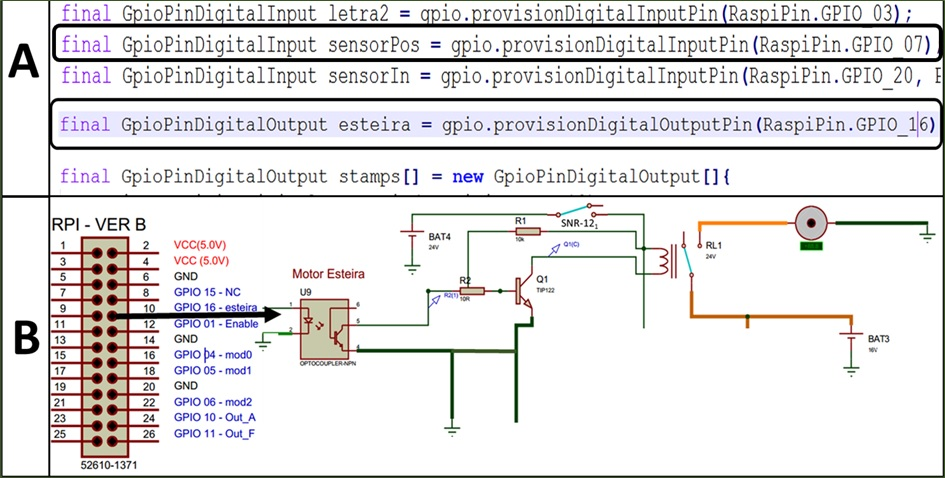
\includegraphics[width=8.9cm, height=7cm]{MeDSE_imagens/F128_SIAPE_SEGURANCA.jpg} 
		\caption{SIAPE: NR-12 Segurança}
		\label{F128}
	\end{figure}	
	
	\item[Requisito RQ12] - O requisito Custos nessa análise está relacionado à área da Economia para expressar a necessidade do cliente em ter os seus produtos competitivos no mercado local e global. Dois fatores são aqui considerados para que o produto seja competitivo: preço e entrega. Os ganhos de tempo nas operações de configuração e ramp up, levarão a reduções de tempo que implicarão na redução dos fatores de produção e o fato do sistema ser evolutivo o capacita a atender pequenas quantidades de produtos e consequentemente, aumentando a competitividade dos produtos produzidos por esse produtor. A agilidade dos sistemas evolutivos em responder às mudanças da demanda não afetam a produção aos níveis praticados hoje por sistemas de ambientes 3.0.
	
\end{description}	


\subsection{Análise e validação dos requisitos RQ13 a RQ15}	

\begin{description}
	\item[Requisito RQ13] - Os primeiros trabalhos de Especificação para a arquitetura da Internet das Coisas \textit{(IoT)} procurou evidenciar especificamente a atualização do estado da arte para questões relacionadas com a Plug \& Play, a partir de um ponto de vista de Internet de Coisas, na fabricação e automação, bem como na aquisição de requisitos funcionais. Essa primeira iteração teve o objetivo de coletar os aspectos mais centrais e críticos de Plug \& Work (Plugar e trabalhar) no ambiente industrial, isto é, num sistema em funcionamento, pode-se incluir um módulo do sistema e esse iniciar imediatamente o seu funcionamento sem causar a necessidade de parar o sistema para realizar essa operação. \par 
	
	A análise relatada  no documento identificou três cenários principais diferentes. Aqui neste trabalho considerou-se especificamente as questões relacionadas no Apêndice B que trata a manufatura ágil. Como Manufatura Ágil o apêndice define uma produção fortemente baseada na disponibilidade da tecnologia de fabricação que pode ser facilmente reconfigurada para responder rapidamente às contínuas mudanças do mercado e continua a fornecer controle total da produção custos e qualidade. \par 
	Como pode ser entendido pela redação o conceito de \textit{plug-and-produce} vai além do conceito de \textit{plug \& work} pois além de plugar e produzir, \textit{plug-and-produce} prevê tanto a inclusão quanto  exclusão de um módulo no sistema sem reduzir a performance do mesmo. Esse conceito foi evidenciado na passagem do produto B para o produto C.	
	
	\item[Requisito RQ14] - A Indústria 4.0 é um conceito que se transforma em realidade com a realização de mudanças no mundo da produção industrial. O aumento exponencial da capacidade dos computadores possibilita a realização de muitos algoritmos até então não realizados pela capacidade das máquinas, a grande quantidade de informação digitalizada e as novas estratégias inovadoras de pessoas, pesquisas e tecnologia concretizam rapidamente esse novo ambiente no globo terrestre.\par 	
	Uma empresa com características da Indústria 4.0 dispõe em sua planta fabril de dispositivos que são reconhecidos de duas formas: A primeira forma por sua estrutura física por meio das máquinas equipamentos e recursos utilizados no mundo real. A outra forma é por sua estrutura virtual, ou seja,  por seus IDs ao entrarem no domínio de uma rede de comunicação. Esses dispositivos uma vez reconhecidos, podem ser configurados e utilizados em sistemas evolutivos com níveis elevados de flexibilidade, plugabilidade, modularidade, escalabilidade, interoperabilidade, agilidade, auto-organização, precisão e outras propriedades comuns aos dispositivos que sofreram a influência da 4a Revolução Industrial. Uma planta formada por módulos mecatrônicos, por dispositivos eletromecânicos, mecânicos e eletrônicos comandados por sistemas de computação baseados em paradigmas de multi-agentes inteligentes pode desempenhar atividades que denotam a inteligência necessária e suficiente para atender às alterações de demanda de produtos dentro de um sistema de manufatura. Somando-se ao atendimento da demanda, o fato da redução de setup a nível que tendem a zero, através da modularidade das partes do sistema, consegue-se a escalabilidade a níveis que atendam a urgência de produção da Customização e tem-se a concretização de sistemas evolutivos como potencial solução do problema de lotes pequenos que tem inviabilizado os atuais sistemas de produção. \par
	
	Num futuro próximo, a instalação de produção reconhecerá por si própria (a esteira e o palete codificado acionado pelo agente AcHw) o que terá de fazer em cada nova peça ou produto. A forma de codificação utilizada poderá variar de acordo com o avanço da tecnologia, no SIAPE a codificação utilizada foi a marcação lateral com hastes metálicas que são detectadas por sensores magnéticos (sA, sF, sM, sT e sU) mas poderia ser na forma de um chip eletrônico, uma identificação para leitura RFID ou até mesmo código de barras. Cada vez mais o produto será fabricado de acordo com os desejos individuais do cliente.
	
	Em outras palavras isto quer dizer, para cada objeto real tem de haver uma imagem virtual para que possa comunicar-se posteriormente com outras máquinas ou peças. As partes real e virtual poderão comunicar-se apenas no nível virtual. No nível virtual são realizadas as operações complexas e tomadas as decisões que demandem inteligência e raciocínio. O resultado é comunicado à parte real que realiza a decisão correta a ser realizada, por exemplo, a produção do estudo de caso. A expansão do mundo virtual cria a possibilidade de comunicação com outras máquinas e sistemas que realizam finalmente o conceito da integração Horizontal recomendada pela Plataforma da Indústria 4.0.
	
	\item[Requisito RQ15] - O estado da arte originado da relação com a Academia foi incluído como forma de evidenciar que os sistemas evolutivos, baseados no paradigma evolutivo é na atualidade, o que existe de mais promissor como solução para o problema da indústria que trata da customização de massa.
	
	A Academia em todo o mundo faz as pesquisas na busca da realização da Indústria 4.0 que requer respostas e soluções para diferentes tópicos como cyber-segurança, padrões aceitáveis e interoperabilidade entre máquinas e sistemas, e sustentabilidade. 
	
\end{description}	



\subsection{Comparações SIAPE versus Produto UFAM}

O plano de produção realizado na experimentação foi expandido para uma quantidade de 10 unidades de produtos. Os tempos decorridos na produção estão registrados na Tabela~\ref{T16}. Todos os tempos em segundos \textbf{(s)}. O tempo médio de palavras com quatro letras realizadas no SIAPE (por exemplo UFAM e UTAM) foi de 10 segundos enquanto a mesma produção realizada no Produto UFAM apresentou uma média de 15 segundos. Para palavras com três letras o SIAPE registrou o tempo de respectivamente de 9 e 10 segundos. O incremento representa um aumento no tempo decorrido de 32\% a mais no Produto UFAM para realizar a mesma produção realizada no SIAPE.

\begin{table}
	\small
	\centering
	\caption{SIAPE X PRODUTO UFAM: TEMPO DE PRODUÇÃO (s)}
	\begin{tabular}{ c|c c| c c | c c }
		\hline
		\textbf{ Palavra} & \multicolumn{1}{c}{\textbf{UFAM}}  & \multicolumn{1}{c}{\textbf{UTAM}} & \textbf{ UEA} & \textbf{ AFM} \\ \hline
		\textbf{Item} & \textbf{SIAPE} & \textbf{PUFAM} & \textbf{ SIAPE} & \textbf{ PUFAM} & \textbf{ SIAPE} & \textbf{ PUFAM}\\ 
		\hline
		
		01 &10,16 &  14,70  & 10,66 & 15,70 & 10,20 &  10,67 \\ \hline
		02 & 10,17 &  16,68  & 10,71 & 14,66 & 9,92  &  10,44 \\ \hline
		03 & 10,88 &  15,59  & 10,49 & 16,50 & 10,30 &  10,56	\\ \hline
		04 & 10,07 &  15,55  & 10,57 & 15,03 & 10,20 &  10,67	\\ \hline
		05 & 10,04 &  15,60  & 10,64 & 15,55 & 10,10 &  10,66	\\ \hline
		06 & 10,72 &  15,60  & 10,72 & 15,04 & 10,10 &  10,45	\\ \hline
		07 & 10,72 &  15,55  & 10,72 & 15,58 & 10,19 &  10,34	\\ \hline
		08 & 10,94 &  14,90  & 10,44 & 14,97 & 15,10 &  10,45	\\ \hline
		09 & 10,91 &  14,94  & 10,71 & 14,95 & 10,20 &  10,67 \\ \hline
		10 & 10,73 &  15,11  & 10,73 & 15,30 & 10,10 &  10,56	\\ \hline
		\hline
		Média & 10,50 &  15,42 	& 10,60 & 15,33 & 9,10 &  10,55	\\ \hline
	\end{tabular}												
	\label{T16}\par
	%	Fonte: Hiram Amaral
\end{table}

Existem alguns motivos que explicam essa vantagem no desempenho do SIAPE em relação ao Produto UFAM. Dois desses motivos estão registrados na Tabela \ref{T17} e são explicados na sequência. \par 

Na segunda coluna da Tabela \ref{T17} estão registrados os dados coletados no SIAPE quando o agente Stamper realiza seu skill carimbar letra. O tempo médio da realização deste skill é de 1 segundo contra 3 segundos registrados na operação das válvulas pneumáticas do Produto UFAM. A diferença em torno de 2 segundos é explicada pelo fato do circuito elétrico do motor DC, utilizado nos módulos do SIAPE, reagir com maior eficácia  quando comparado ao circuito eletro-pneumático do Produto UFAM, pois o circuito só reage, primeiramente com os solenóides, e depois os solenóides liberam as válvulas pneumáticas que realizam a operação carimbar letra. Esses tempos reduzem o desempenho do produto UFAM para esse nível de produção nas condições aqui consideradas.\par

Outro motivo que reduz também o desempenho do Produto UFAM para as condições apresentadas é o fato do sistema ter sido projetado para que o operador aguarde a finalização do produção de um produto e reinsira o palete na entrada do sistema. Essa operação registrou um tempo médio de 3 segundos contra 1 segundo do SIAPE. No SIAPE os paletes já encontram-se agregados à esteira, cabendo ao operador apenas retirar os produtos realizados. 

As colunas 6 e 7 da Tabela \ref{T17} registra os tempos com a troca de módulos com o SIAPE em funcionamento. O tempo médio para realizar a troca de um módulo pelo operador, com a detecção deste pelo agente AcHw e posterior inclusão do novo recurso no plano de produção alcançou a média de 45 segundos. Vale registrar que esse tempo iniciou-se em torno de 4 minutos que foi reduzido para 2 minutos até alcançar o tempo atual registrado. Apesar do tempo reduzido este processo que realiza o \textit{plug and produce} pode ser reduzido ainda mais por meio de melhorias no hardware.  A sétima coluna registra o fato dessa mesma operação ser realizada no Produto UFAM, dado que os procedimentos exigiriam a parada do sistema elétrico e do sistema pneumático para posterior troca mecânica da válvula pneumática.



%%%

\begin{table}[!h]
	\centering
	\caption{SIAPE X PRODUTO UFAM: STAMPER, OPERADOR e TROCA(s)}
	\footnotesize
	\begin{tabular}{C{1cm} | C{1cm} C{1cm} | C{1cm} C{1cm} | C{1cm} C{1cm}} 
		\hline
		\textbf{Item} & \textbf{SIAPE Stamper} & \textbf{PUFAM Stamper} & 
		\textbf{SIAPE Operador} & \textbf{PUFAM Operador} & \textbf{SIAPE Troca} & \textbf{PUFAM Troca} \\
		
		\hline
		\hline
		01  & 1,79 & 3,30 & 1,89 & 3,06 & 48,73 &  \multirow{11}{*}{\begin{sideways}I m p r a t i c á v e l\end{sideways}} \\ \cline{1-6}
		02  & 1,87 & 2,86 & 1,89 & 2,83 & 46,25 &  \\ \cline{1-6}
		03  & 1,64 & 3,50 & 1,86 & 3,20 & 49,25 &  \\ \cline{1-6}
		04  & 1,72 & 4,19 & 1,62 & 3,39 & 50,25 &  \\ \cline{1-6}
		05  & 1,88 & 3,42 & 1,95 & 3,50 & 42,65 &  \\ \cline{1-6}
		06  & 1,76 & 3,50 & 1,98 & 4,01 & 43,25 &  \\ \cline{1-6}
		07  & 1,67 & 3,51 & 1,87 & 3,09 & 44,50 &  \\ \cline{1-6}
		08  & 1,54 & 3,80 & 1,89 & 3,55 & 46,20 &  \\ \cline{1-6}
		09  & 1,67 & 3,86 & 1,87 & 2,86 & 43,25 &  \\ \cline{1-6}
		10  & 1,88 & 3,64 & 1,88 & 3,22 & 44,30 &  \\ \cline{1-6}
		\hhline{======}
		Média & 1,74 & 3,56 & 1,90 & 3,27 & 45,86 &  \\ \hline
		
	\end{tabular}												
	\label{T17}\par
	%	Fonte: Hiram Amaral
\end{table}




\begin{table}
	\small
	\centering
	\caption{SIAPE X PRODUTO UFAM: TEMPO DE PRODUÇÃO(s)}
	\begin{tabular}{c c | c c | c c | c c | c}
		\multicolumn{2}{c|}{\textbf{Item}} & 
		\textbf{PUFAM} & \textbf{SIAPE} & 
		\textbf{PUFAM} & \textbf{SIAPE} & 
		\textbf{PUFAM} & \textbf{SIAPE} &
		\multirow{2}{*}{$\Delta\%$} \\
		
		\textbf{PROD} & \textbf{QTD} & 
		\multicolumn{2}{c|}{\textbf{t\underline{ }TOTAL}} &
		\multicolumn{2}{c|}{\textbf{t\underline{ }CICLO\underline{ }P}} &
		\multicolumn{2}{c|}{\textbf{t\underline{ }CICLO\underline{ }O}} &
		~ \\ \hline \hline
		
		A &  3  & 46,97 & 31,21  & 15,657 & 10,403 &  5,219  &  3,468 & 33,55 \\
		\hline
		
		B &  4  & 61,89 & 42,43  & 15,473 & 10,608 &  3,860  &  2,652 & 31,44 \\
		\hline
		
		C &  5  & 53,00 & 50,65  & 10,600 & 10,130 &  2,120  &  2,026 &  4,43 \\
		
		
	\end{tabular}
	\label{T19}\par
	%	Fonte: Hiram Amaral
\end{table}

A análise da Tabela \ref{T19} evidencia que o aumento de lotes  de produção têm vantagens consideráveis para serem realizadas no Produto UFAM. Isso se deve ao fato do produto UFAM não utilizar uma plataforma de agentes inteligentes como ocorre com o SIAPE. Não utilizando agentes, não há necessidade do uso de protocolos de comunicação FIPA. Não havendo comunicação, o tempo reduz-se consideravelmente, refletindo em vantagens para o uso do Produto UFAM. Assim para lotes médios e altos os sistemas flexíveis ainda são uma alternativa rentável, contudo, para pequenos lotes com alta variedade de produtos, os sistemas ágeis e evolutivos são realmente uma excelente alternativa, principalmente, para tratar o problema da customização em massa.


\subsection{Considerações finais}

O SIAPE, desenvolvido pelo Método de Desenvolvimento de Sistemas Evolutivos - MeDSE trilhou um procedimento sistematizado para ficar aderente ao paradigma \textit{EPS}, e por conseguinte, aderente à Plataforma da Indústria 4.0. O fato de ser baseado no Produto UFAM com características de sistemas utilizados no parque industrial brasileiro, evidenciou a possibilidade de transformar um sistema de ambiente 3.0 num sistema ágil evolutivo com as principais características do paradigma EPS que promete tratar o problema da customização de massa.

Desde as etapas mais básicas do MeDSE, o conceito de \textit{skill} foi considerado. O problema Global foi gradativamente refinado em problemas regionais e locais, com características atômicas, necessárias para a modelagem dos módulos com a granularidade adequada ao sistema desenvolvido, que no caso do SIAPE optou-se por uma granularidade grossa por definir anagramas completos a serem realizados e  não partes desses. A granularidade fina para o caso do SIAPE implicaria na implementação de um grupo de agentes que ficasse responsável por partes de uma letra, por exemplo para realizar a letra E dois agentes cognitivos que  acionassem dois módulos com os símbolos '|' e '\_'  seriam necessários. A granularidade grossa, de fato, foi o suficiente para atingir as metas do SIAPE.

Da modelagem seguiu-se as simulações que garantiram os circuitos e modelos como especificações que foram organizadas e receberam o status de projeto de sistema. O projeto foi realizado seguindo o restante das  etapa definidas no MeDSE e sistema foi transformado num produto. Com a experimentação e as comparações evidenciou-se, entre outros, os parâmetros que classificam o SIAPE como um sistema evolutivo, e com melhor desempenho que o Produto UFAM nas situações que demandam maior agilidade e flexibilidade em tempo real. É importante notar também que o paradigma EPS é melhor para aplicações em contextos que demandem maior agilidade e robustez para lidar com alterações na demanda. Essas alterações são tratadas imediatamente pela capacidade do sistema da adaptação, no longo prazo tendem à evolução dos sistemas que detém tais características. Não fossem essas necessidades os sistemas flexíveis dos ambientes 3.0 ainda seriam uma solução robusta e satisfatória para tratar o problema da produção mundial.   




%==========================================


% SEÇÃO VI
\section{CONCLUSÃO}
Este artigo apresentou os princípios básicos da Metodologia para Desenvolvimento de Sistemas Evolutivos - MeDSE e realizou
uma aplicação da metodologia a um sistema denominado de SIAPE. Além da verificação dos princípios básicos da metodologia, pode-se evidenciar a possibilidade de seguir gradativamente os procedimentos nos projetos parciais e se pôde acompanhar todos os desenvolvimentos, testes e simulações
individuais que capacita os projetistas a dominarem de uma forma mais completa (circuitos elétricos, mecânicos, códigos de
software e os sistemas de comunicação utilizados pelo sistema como um todo) . \par

Com a implementação evidenciou-se, a classificação do SIAPE como um sistema evolutivo em situações que demandam maior agilidade e flexibilidade em tempo real. É importante notar também que o paradigma EPS é melhor para aplicações em contextos que demandem maior agilidade e robustez para lidar com alterações na demanda. Essas alterações são tratadas imediatamente pela capacidade do sistema da adaptação. No longo prazo tendem à evolução dos sistemas que detém tais características. 
Como trabalho futuro espera-se realizar uma experimentação que se possa seguir todos os procedimentos da metodologia, e que se possa evidenciar o desenvolvimento de hardware e software que compõem o sistema.

% SEÇÃO VII
\section{AGRADECIMENTOS}

Nossos agradecimentos à FAPEAM, UFAM e CETELI

\textit{Part of the results presented in this paper were obtained via the project for research and human resources quali
- cation, under- and post-graduate levels, in the areas of industrial automation, mobile devices software, and Digital TV,
sponsored by Samsung Eletronica da Amazonia Ltda, under the terms of Brazilian Federal Law number 8.387/91.}


%=========================== REFERÊNCIAS ==========================


\begin{thebibliography}{99}
	%=========================== 1 customização ===========================
	\bibitem{E.Abele}E. Abele, 
	\emph{"Global Production: A hand book of Strategy and Implementation,"} Springer, 2008. [Online]. Available: http://books.google.co.uk/books?id=baQOlzVEmuAC\&printsec. [Accessed: 01-Feb-2015].
	%============================= 2  EPS =============================		
	\bibitem{A.Rocha} A. Rocha, L. Ribeiro and J. Barata,
	\emph { "A Multi Agent Architecture to Support Self-organizing Material Handling," )}, Technological Innovation for Collective 2014.
	%============================ 3 IoT ==============================		
	\bibitem{A.Whitmore} A. Whitmore, A. Agarwal, and L. Da Xu, 
	\emph{ " The Internet of Things-A survey of topics and trends," }, Inf. Syst. Front., pp. 1--14, 2014.
	
	%=============== 4 FMS  ================
	\bibitem{FMS}H. ElMaraghy, 
	\emph{"Flexible and reconfigurable manufacturing systems paradigms,} Flex. Serv. Manuf. J., vol. 17, pp. 261--276, 2006.
		
	%====================5 6  BMS ===========================
	
	%	[23]	J. Vaario, K. Ueda, and R. Nada, ?Biological concept of self-organization for dynamic shop-floor configuration,? 1998.
	\bibitem{BMS} K. Ueda, 
	\emph{"A Concept for Bionic Manufacturing Systems Based on DNA-type Information. BT"} -- PROLAMAT Conference, Man in CIM. Tokyo, Japan, 24-26 June 1992.- pp. 853-863, 1992.
	
	\bibitem{J.Ferreira} J. Dias Ferreira, L. Ribeiro, M. Onori, and J. Barata, 
	\emph{"Bio-inspired Self-Organising Methodologies for Production Emergence,} in Systems, Man, and Cybernetics (SMC), 2013 IEEE International Conference on, 2013, pp. 3835?3841.
	
	%============================7 e 8  9 HMS  ============================	

	\bibitem{Christensen}James H. Christensen,
	\emph{"Holonic Manufacturing ystem: Initial architecture and standards directions"}, Presented at First European Conference on Holonic Manufacturing Systems, Hannover, Germany, 1 December 1994., no. March, pp. 1-- 20, 1994. 

	\bibitem{Christensen} J. H. Christensen, 
	\emph{"HMS / FB Architecture and its Implementation"}, Agent-based Manuf. Adv. holonic approach, pp. 53--83, 2003.	
				
	\bibitem{VanBrussel}H. Van Brussel, J. Wyns, P. Valckenaers, L. Bongaerts, and P. Peeters, \emph{"Reference architecture for holonic manufacturing systems: PROSA"}, Comput. Ind., vol. 37, pp. 255?274, 1998.
	
	%================ 10 RMS ==================
	\bibitem{RMS}Y. Koren, U. Heisel, F. Jovane, T. Moriwaki, G. Pritschow, G. Ulsoy, and H. Van Brussel, 
	\emph{"Reconfigurable Manufacturing Systems"}, vol. 48, pp. 527--540, 1999.
	
	%=============================== 11 12 13 14EAS/EPS ======================================			
	\bibitem{M.Onori_a}
	\emph{	M. Onori, "Evolvable Assembly Systems -- A New Paradigm?", Proc. 33rd Int. Symp. Robot., pp. 617--622, 2002.},
	
	\bibitem{M.Onori_b} M. Onori, J. Barata, and R. Frei, 
	\emph {"Evolvable assembly systems basic principles"}, Inf. Technol. Balanc. Manuf. Syst., vol. 220, pp. 1--12, 2006.
	
	\bibitem{L.Ribeiro}L. Ribeiro and J. Barata,			
	\emph {"IMS 10--Validation of a co-evolving diagnostic algorithm for evolvable production systems,"} Eng. Appl. Artif. Intell., vol. 25, no. 6, pp. 1142--1160, Sep. 2012.
		
	\bibitem{AMaffei}A. Maffei and M. Onori,
	\emph{{A preliminary study of business model for evolvable production systems}}, in Assembly and Manufacturing, ISAM 2009, IEEE International Symposium on, 2009, pp. 402--407.
	
	%============================ 15 MAS =============================

		\bibitem{P. Leitao}V. Marik, P. Vrba, and S. Member,
		\emph{ Past, Present, and Future of Industrial Agent Applications, Ind. Informatics, IEEE Trans., vol. 9, no. 4, pp. 2360--2372, 2013.}
	%============================ 16 IoT =============================
				
	\bibitem{ROTONDI} D. ROTONDI, S. Piccione, G. Altomare, A. M. Houyou, J. Gessner, C. Kloukinas, K. Mahbub, and H. Trsek,
	\emph{"IoT \@ Work WP 1 -- PLUG\&WORK IOT REQUIREMENT ASSESSMENT AND ARCHITECTURE D1.3}   pp. 1--135, 2013.		
	%============================ 17 EPS =============================
				
	\bibitem{A.L.D.Cavalcante} A. L. D. Cavalcante,
	\emph{"Arquitetura baseada em agentes e auto-organizável para a manufatura,"} Porto Alegre, 2012.
	%============================ 18 i4.0 =============================		

	\bibitem{DRATH2014} DRATH, Rainer and Horch, Alexnder,
	\emph{{Industrie 4.0: Hit or hype-- [Industry Forum]}}, IEEE Industrial Electronics Magazine, 	Doi {10.1109/MIE.2014.2312079}, 2014.	
	%============================ 19 H2020 =============================
	
	\bibitem{H2020}E. Commission, 
	\emph{"EU - A Strategy for smart, sustainable and inclusive growth 2010-2020"}, in COMMUNICATION FROM THE COMMISISON -EU, 2010.
	%============================ 20 21 23 CPS =============================

	\bibitem{B.Krogh} B. Krogh, E. Lee, I. Lee, a Mok, and R. Rajkumar, 
	\emph{"Cyber-Physical Systems, Executive Summary,"} Sci. Technol., 2008.

	\bibitem{L.Monostori} L. Monostori, 
	\emph{"Cyber-physical production systems: Roots, expectations and R\&D challenges,"} Procedia CIRP, vol. 17, pp. 9--13, 2014.

\bibitem{NITRD}NITRD, 
\emph{"Cybersecurity Game-Change Research \& Development Recommendations"},  pp. 1--18, 2010.

	%============================ 24 i4.0 =============================
			
	\bibitem{VDE2014}German Commission for Electrical,
	\emph{"DKE standardization the german standardization roadmap"}, German Commission for Electrical VDE, Electronic \& Information Technologies of DIN, 2014.					
					
	%============================ 25 HMS =============================			
		
	\bibitem{J.Barbosa}	J. Barbosa, P. Leitao, E. Adam, and D. Trentesaux, \emph{ "Self--Organized Holonic Multi-agent Manufacturing System: The Behavioural Perspective,"} in Systems, Man, and Cybernetics (SMC), 2013 IEEE International Conference on, 2013, pp. 3829--3834.


%================= 28  Humbolditiano =========================
\bibitem{F.Lemos}F. Lemos, 
\emph{"[Sobre reformas no sistema de ensino] Wilhelm von Humboldt,} Rev. Bras. História da Educ., vol. 11, no. 1(25), pp. 207--241, 2011.

%================= 29 Triplice Helice =========================

\bibitem{R.M.Rossa}R. M. Rossa, J. R. Garcia, and A. G. R. Lezana, 
\emph{"A abordagem hélice tríplice das relações entre universidade-indstria-governo"},  Simpoi 2013, pp. 1--16, 2013.	
%============  30 Academia ===============			
\bibitem{CAPES}CAPES - Volume I, 
\emph{"Programa Nacional Pós-Graduação ( Pnpg ) 2010-2020}, vol. I. 2011.

%=============== 31 Governo =================
\bibitem{C.Civil}	Casa Civil, 
\emph{"Decreto 8269 - Plataformas de Conhecimento - Presidência da República"}, pp. 2--5, 2014.
%=============== 32 Indústria  ================
\bibitem{CNI}Confederação Nacional da Indústria - CNI,
\emph{"Mapa Estratégico Mapa (2013 - 2022)"}. 2013.

	%========================= Metodologia ==========================
	%33
	\bibitem{Meyer}B. Meyer,
	\emph{"Object-Oriented Software Construction "}, Nucl. Instruments Methods Phys. Res. Sect. A Accel. Spectrometers, Detect. Assoc. Equip., vol. 352, p. 1300, 2000.
		
	%[34]	
	\bibitem{RUMBAUGH} J. RUMBAUGH, 
	\emph{" Object-Oriented Modeling and Design"}, 1991.	
	
	\bibitem {LARMAN2007}Larman Craig,
	\emph{Utilizando UML e padrões: Uma introdução à análise e ao projeto orientado a objetos e ao desenvolvimento iterativo}, Tradução de Rosana Vaccare Braga [et al.], 2007
	
	%[35]
	\bibitem{BOOCH}Grady Booch ,
	\emph{" Object-Oriented Design with Applications "}, Benjamin/Cummings, Redwood City, CA, 1991.	
	
	%[36]
	\bibitem{JACOBSON} Jacobson, M. Christerson, P. Jonsson, and G. Overgaard.,
	\emph{"Object-Oriented Software Engineering. A Use Case Driven Approach. ACM Press, 1992. "}, 1992.
		
	%[37]	
	\bibitem{RATIONAL} Rational Software Corporation.,
	\emph{"Unified Modelling Languaje (UML) version 1.0. Rational Software Corporation, 1997 "},1997 .
		
	%[38]	
	\bibitem{SHOHAM} Y. Shoham ,
	\emph{" Agent-oriented programming, "}, vol. 60, pp. 51?92, 1993.
		
	%[39]
	\bibitem{KINNY} Kinny; Georgeff; Rao, ,
	\emph{"A Methodology and Modelling Technique for Systema of BDI Agents, "},1996 .
		
	%[40]	
	\bibitem{BURMEISTER} B. Burmeister,
	\emph{"Models and methodology for agent-oriented analysis and design, "}, Work. Notes KI, vol. 96, no. i, pp. 96?06, 1996.
		
	%[41]
	\bibitem{DELOACH}Scott a. deloach, mark f. wood and clint h. sparkman, ,
	\emph{" Introduction. J. Software. Engineering. Knowlegde. "}, vol. 11, no. 3, pp. 231?258, 2001..
		
	%[42]	
	\bibitem{CAIRE} Caire,
	\emph{"Technical Information MESSAGE?: Methodology for Engineering Systems of Software Agents, "}, no. September 2001, 2001.
	
	%[43]
\bibitem{BRESCIANI}Bresciani et.al.
\emph{"Tropos: An Agent-Oriented Software Development Methodology, "}, Auton. Agent. Multi. Agent. Syst., vol. 8, pp. 203?236, 2004..

%44
\bibitem{ZAMBONELLI}Zambonelli, Jennings e Wooldridge
\emph{"Developing Multiagent Systems: The Gaia Methodology "}, ACM Transactions on Software Engineering and Methodology, Vol. 12, No. 3, July 2003, Pages 317–370..

%45
\bibitem{RIBEIRO2008} Ribeiro, L., Barata, J., and Colombo, A.
\emph{ MAS and SOA: A case study exploring principles and technologies to support self-properties }, in assembly systems. Proceedings - 2nd IEEE International Conference on Self-Adaptive and Self-Organizing Systems Workshops, SASOW 2008, 192–197. doi:10.1109/SASOW.2008.
%46
\bibitem{BITKOM2015}BITKOM, VDMA \& ZVEI,
\emph{Whitepaper FuE-Themen }, http://www.plattform-i40.de/blog/industrie-40-whitepaper-fue-themen-stand-7-april-2015, p. 59,2015
%47
\bibitem{ROSA2013c}ROSA, RPG,
\emph{Assessing self-organization and emergence in Evolvable Assembly Systems (EAS)}, 2013.
%48
\bibitem {ATKINS} Atkins,
\emph{Revolutionizing Science and Engineering Through Cyberinfrastructure}, Report of the National Science Foundation Blue-Ribbon Advisory Panel, 2003.		
%49
\bibitem {FERREIRA} P. Ferreira, N. Lohse, M. Razgon, P. Larizza, and G. Triggiani, 
emph{Skill based configuration methodology for evolvable mechatronic systems}, in IECON 2012 - 38th Annual Conference on IEEE Industrial Electronics Society, 2012, pp. 4366?4371.		

%============================== CPS ================================
	%	[32]	R. Frei, J. Barata, and M. Onori, ?Evolvable production systems context and implications,? IEEE Int. Symp. Ind. Electron., vol. 00, pp. 3233?3238, 2007.
	%[50]	M. Onori, J. Barata, and R. Frei, ?Evolvable assembly systems basic principles,? Inf. Technol. Balanc. Manuf. Syst., pp. 1?12, 2006.

		%[54]	A. Connect, ?? Smart Cyber-Physical Systems ,?? 2014.
		%[55]	C. Laschi, T. U. M. De, K. Ridgway, U. Z. H. Ch, M. Althoff, A. De, D. Scaramuzza, I. I. T. It, and D. Caldwell, ?S \& T QUALITY.?


	%[57]	D. ROTONDI, S. Piccione, G. Altomare, A. M. Houyou, J. Gessner, C. Kloukinas, K. Mahbub, and H. Trsek, ?IoT @ Work WP 1 ? PLUG\&WORK IOT REQUIREMENT ASSESSMENT AND ARCHITECTURE D1.3 ? Final framework architecture specification,? pp. 1?135, 2013.
	%[58]	NIC-USA, ?IoT - SIX DISTUPTE TECHNOLOGIES,? pp. 1? 48, 2008.
	%[59]	H. Zou, H. Wang, L. Xie, and Q.-S. Jia, ?An RFID indoor positioning system by using weighted path loss and extreme learning machine,? in 2013 IEEE 1st International Conference on Cyber-Physical Systems, Networks, and Applications (CPSNA), 2013, pp. 66?71.
		
	
	%[48]	S. Tripakis, C. Stergiou, C. Shaver, and E. a Lee, ?A modular formal semantics for Ptolemy,? Math. Struct. Comput. Sci., vol. 23, pp. 834?881, 2013.
	
	
	

	%[6]	C. Yu, M. Zhang, S. Member, F. Ren, and G. Tan, ?Multiagent Learning of Coordination in Loosely Coupled Multiagent Systems,? pp. 1?15, 2015.
	%[7]	V. M. Catterson, E. M. Davidson, and S. D. J. McArthur, ?Practical applications of multi-agent systems in electric power systems,? Eur. Trans. Electr. Power, vol. 22, no. 2, pp. 235?252, 2012.
	
	%[68]	Y. Koren, U. Heisel, F. Jovane, T. Moriwaki, G. Pritschow, G. Ulsoy, and H. Van Brussel, ?Reconfigurable Manufacturing Systems,? CIRP Ann. - Manuf. Technol., vol. 48, pp. 527?540, 1999.
	%[66]	ERA_EUROPEAN_COMISSION, ?A Reinforced European Research Area Partnership for Excellence and Growth,? 2012.
	%[67]	P. Lines, ?Scope and findings?:,? no. January, 2015.
	
	%========================= SKILL ================================
	%[64]	P. Leitao, V. Marik, P. Vrba, and S. Member, ?Past, Present, and Future of Industrial Agent Applications,? Ind. Informatics, IEEE Trans., vol. 9, no. 4, pp. 2360?2372, 2013.
	%1]	P. Deusdado, G. Candido, and J. Barata, ?Dynamic skills composition and execution in a Multi-agent Manufacturing System,? in Industrial Electronics (ISIE), 2011 IEEE International Symposium on, 2011, pp. 1785?1790.

	%============================ ICT ===============================
	
	
		%========================= CPS ================================
		%[48]	S. Tripakis, C. Stergiou, C. Shaver, and E. a Lee, ?A modular formal semantics for Ptolemy,? Math. Struct. Comput. Sci., vol. 23, pp. 834?881, 2013.
		%[51]	H. Gill, ?Challenges for critical embedded systems,? Proc. - Int. Work. Object-Oriented Real-Time Dependable Syst. WORDS, pp. 7?9, 2005.
		%[52]	J. C. Eidson, E. A. Lee, S. Matic, S. A. Seshia, and Z. Jia, ?Distributed Real-Time Software for Cyber \&\#x2013;Physical Systems,? Proc. IEEE, vol. 100, no. 1, pp. 45?59, 2012.
		
		
		%	\bibitem{A.Maffei}
		%	\emph{A. Maffei, H. Akillioglu, and L. Flores, "Characterization of Costs and Strategies for Automation in Evolvable Production Systems," , 2013, pp. 4866?4871.}

	
	%[6]	C. Yu, M. Zhang, S. Member, F. Ren, and G. Tan, ?Multiagent Learning of Coordination in Loosely Coupled Multiagent Systems,? pp. 1?15, 2015.
	%[7]	V. M. Catterson, E. M. Davidson, and S. D. J. McArthur, ?Practical applications of multi-agent systems in electric power systems,? Eur. Trans. Electr. Power, vol. 22, no. 2, pp. 235?252, 2012.
	
	%[68]	Y. Koren, U. Heisel, F. Jovane, T. Moriwaki, G. Pritschow, G. Ulsoy, and H. Van Brussel, ?Reconfigurable Manufacturing Systems,? CIRP Ann. - Manuf. Technol., vol. 48, pp. 527?540, 1999.
	%[66]	ERA_EUROPEAN_COMISSION, ?A Reinforced European Research Area Partnership for Excellence and Growth,? 2012.
	%[67]	P. Lines, ?Scope and findings?:,? no. January, 2015.
	

	%========================= SKILL ================================
	%[64]	P. Leitao, V. Marik, P. Vrba, and S. Member, ?Past, Present, and Future of Industrial Agent Applications,? Ind. Informatics, IEEE Trans., vol. 9, no. 4, pp. 2360?2372, 2013.
	%1]	P. Deusdado, G. Candido, and J. Barata, ?Dynamic skills composition and execution in a Multi-agent Manufacturing System,? in Industrial Electronics (ISIE), 2011 IEEE International Symposium on, 2011, pp. 1785?1790.
	%[2]	P. Ferreira, N. Lohse, M. Razgon, P. Larizza, and G. Triggiani, ?Skill based configuration methodology for evolvable mechatronic systems,? in IECON 2012 - 38th Annual Conference on IEEE Industrial Electronics Society, 2012, pp. 4366?4371.
	%============================ ICT ===============================


	%=========================== IoT ================================
	%[60]	N. Bui, C. Jardak, and C. Magerkurth, ?Internet-of-Things Architecture IoT-A Deliverable D1.3 ? Updated reference model for IoT v1.5,? no. 257521, pp. 1?256, 2013.
	%[61]	A. Salinas, F. I. Release, R. By, A. S. Segura, and D. Level, ?Internet of Things Architecture Project Deliverable D6 . 1 - Requirements List,? Architecture, no. 257521, 2013.
	%[62]	J. Gubbi, R. Buyya, S. Marusic, and M. Palaniswami, ?Internet of Things (IoT): A vision, architectural elements, and future directions,? Futur. Gener. Comput. Syst., vol. 29, no. 7, pp. 1645?1660, 2013.
	%[63]	V. VYATKIN, ?IEC 61499 as Enabler of Distributed and Intelligent Automation: State-of-the-Art Review,? Ind. Informatics, IEEE Trans., vol. 7, no. 4, pp. 768?781, 2011.
	%[65]	M. R. Van Kranenburg, ?IoT - A Community Newsletter \# 7 Foreword by Thibaut Kleiner,? pp. 1?12, 2013.
	%[5]	O. Said and M. Masud, ?Towards internet of things: Survey and future vision,? Int. J. Comput. Networks, vol. 5, no. 5, pp. 1?17, 2013.
	%[8]	A. Whitmore, A. Agarwal, and L. Da Xu, ?The Internet of Things-A survey of topics and trends,? Inf. Syst. Front., pp. 1?14, 2014.
	%[9]	S. Li, L. Da Xu, and S. Zhao, ?The internet of things: a survey,? Inf. Syst. Front., 2014.
	%[10]	J. A. Stankovic, ?Research Directions for the Internet of Things,? IEEE Internet Things J., vol. 1, no. 1, pp. 1?1, 2014.
	
		
		%================= IEC61499  ==========================
		%	\bibitem{61499}J. Christensen and T. Strasser, ?The IEC 61499 Function Block Standard: Overview of the Second Edition, ISA Autom. , 2012. 
		%======================== === CPS === ==========================			
		
	%================= 26 27 Indústria 4.0  ==========================
	%\bibitem{Nitrdgroups}Nitrdgroups (CPS) Vision Statement, 
	%	\emph{"Cyber Physical Systems (CPS) Vision Statement"} 2012.
	%
	%	\emph{"Exploring the network dimension of diagnosis in Evolvable Production Systems"}, in Emerging Technologies and Factory Automation (ETFA), 2010 IEEE Conference on, 2010, pp. 1--6.
	%		
	%	\bibitem{J.C.Jensen}J. C. Jensen, D. H. Chang, and E. A. Lee, 
	%	\emph{"A model-based design methodology for cyber-physical systems"}, 2011, pp. 1666--1671.
	%	
	%	\bibitem{NFS}National Science Foundation -NFS, 
	%	\emph{"Cyber-Physical Systems PROGRAM SOLICITATION NSF 15--541 REPLACES DOCUMENT ( S )"} pp. 1--20, 2014.
%=============== EMBRAPII ============================
%\bibitem{Julio}K. Julio and C. Pereira, 
%\emph{"EMBRAPII Relatório 2014"}, Associação Brasileira de Pesquisa e Inovação Industrial. - EMBRAPII, 2014.

%======================= 26 27 Horizon 2020 ===========================		
%\bibitem{UE}E. Technologies, 
%\emph{"A guide to ICT-related activities in WP2014-15"}, 2014.
%
%\bibitem{J.Imtiaz}	J. Imtiaz and J. Jasperneite,
%\emph{ "Scalability of OPC-UA down to the chip level enables Internet of Things"} in Industrial Informatics (INDIN), 2013 11th IEEE International Conference on, 2013, pp. 500--505.


\end{thebibliography}


\end{document}


